\documentclass[aspectratio=43]{beamer}
\usetheme{CCNU}
%\usefonttheme[onlymath]{serif}

\usepackage{slashed}
\usepackage{datetime}
%\usepackage{slidesphysics}
\graphicspath{{../img/}}

\usepackage{media9}
\addmediapath{./Movies/}

\usepackage{multimedia}

\usepackage{hyperref}
\usepackage{cancel}
% \hypersetup{colorlinks=true, 
%     linkcolor=blue,          % color of internal links (change box color with linkbordercolor)
%     citecolor=black,        % color of links to bibliography
%     filecolor=black,      % color of file links
%     urlcolor=blue    }
% \usepackage{deflamb}
% \usepackage{color, colortbl}
% \usepackage{tikz}
%\usepackage{userdef}
\usepackage[absolute,overlay]{textpos}
\def\Put(#1,#2)#3{\leavevmode\makebox(0,0){\put(#1,#2){#3}}}

\def\mydate{\leavevmode\hbox{\the\year-\twodigits\month-\twodigits\day}}
\def\twodigits#1{\ifnum#1<10 0\fi\the#1}

\newcommand\Wider[2][3em]{%
\makebox[\linewidth][c]{%
  \begin{minipage}{\dimexpr\textwidth+#1\relax}
  \raggedright
  \centering#2
  \end{minipage}%
  }%
}

%\def\meetingname{Alicia Garrido Peña. PhD thesis Presentation}


\def\meetingname{Alicia Garrido Peña. PhD thesis Seminar}

\title[\meetingname]{Characterization of the sequential nature of neuronal dynamics: Experimental recordings, computational models and novel stimulation neurotechnologies}
\author[A. Garrido-Peña]{Alicia Garrido Peña}
% \institute[Michigan]{}
\institute[UAM]{Universidad Autónoma de Madrid}
\date[\mydate]{\meetingname\\\today}

\begin{document}
	
% Set up the section page style
\AtBeginSection[]{
	\begin{frame}
		\centering
		\Huge \insertsection
	\end{frame}
}

	
	
\begin{frame}[plain,t]
\titlepage
\end{frame}

%The next statement creates the title page.
\begin{frame}
\frametitle{Contents}
\tableofcontents
\end{frame}
%------------------------------------------------------------
\section{Introduction}
\begin{frame}{Neuroscience}
	\only<1>{\includegraphics[width=\textwidth]{intro/neurosciences.pdf}}
	\only<2>{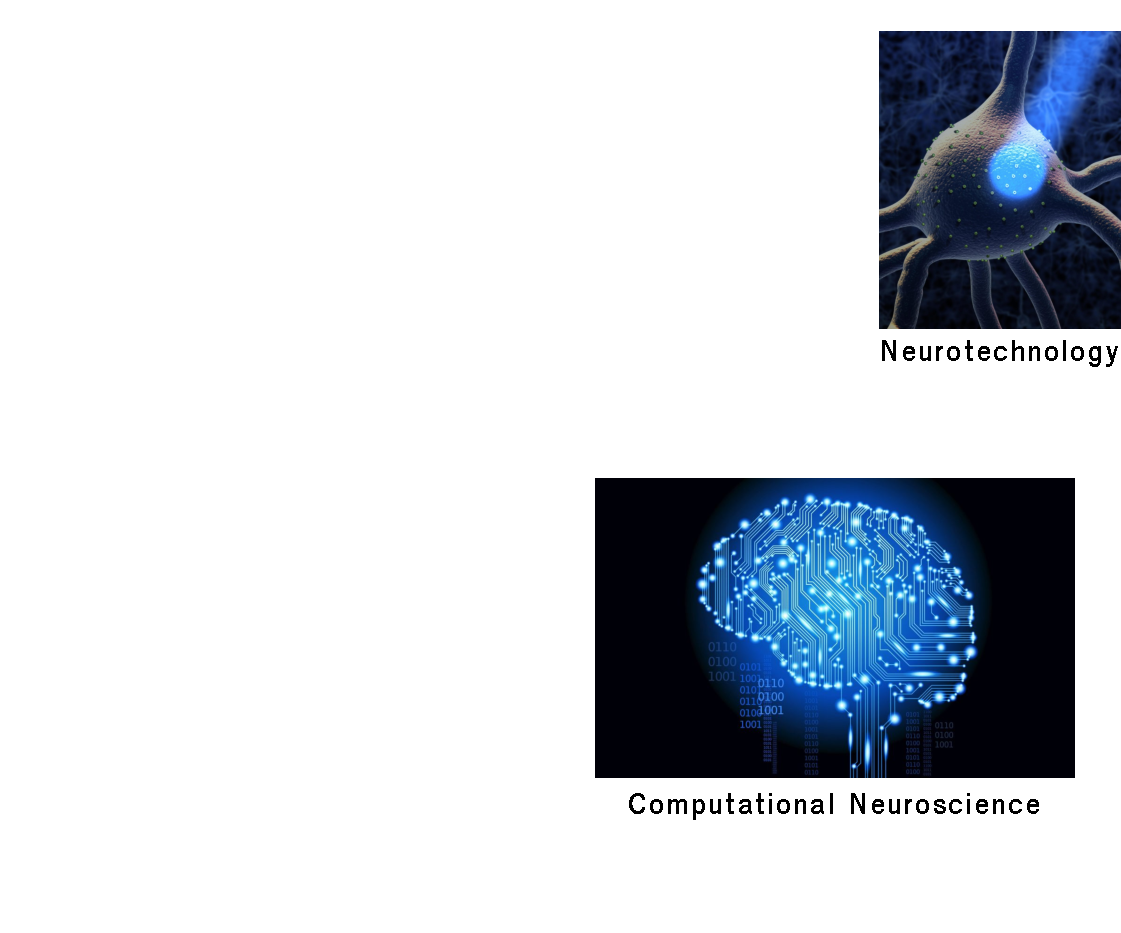
\includegraphics[width=\textwidth]{intro/neurosciences_focus.pdf}}
\end{frame}
\begin{frame}{Approach}
	\begin{itemize}
		\item Neurocomputational Perspective
		\item<2-> Bottom-up approach
		\item<5-> Combining electrophysiology \uncover<6>{and computational work}
	\end{itemize}
	\vfill
	\centering
	\uncover<3-4>{
\includegraphics[width=0.3\textwidth]{intro/ions.pdf}}
	\hspace{30pt}
	\uncover<4-4>{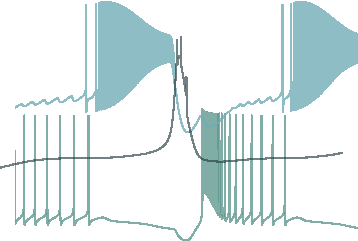
\includegraphics[width=0.4\textwidth]{intro/CPG.pdf}}
	\uncover<3-4>{\\From ionic channels}
	\uncover<4-4>{\hspace{50pt} To minimal circuits}
\end{frame}

\begin{frame}{Neuronal and Networks Dynamics}
	\only<1>{Neuronal electrical activity is often described in terms of the evolution of membrane voltage caused by the flow of ionic channels between the inside and outside of the cell.}
	
	\uncover<2->{Depending on the channels that constitute the neuron and the circuit it is immersed in, the activity varies.}
	\vfill
	\uncover<3->{In terms of the spike waveform:}
	\uncover<3->{\begin{center}
			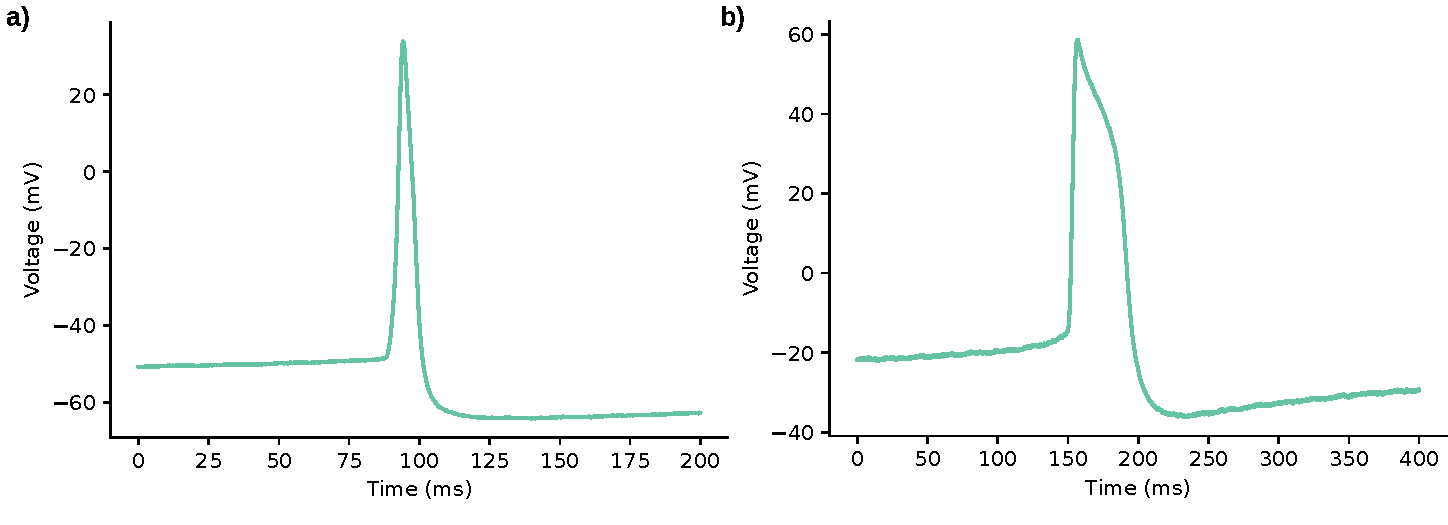
\includegraphics[width=0.7\textwidth]{intro/spike-types.pdf}
	\end{center}}
	
	\uncover<4->{\vfill}
	\uncover<4->{And the type of spiking activity: tonic firing, bursting, etc.}
	\uncover<4->{\begin{center}
			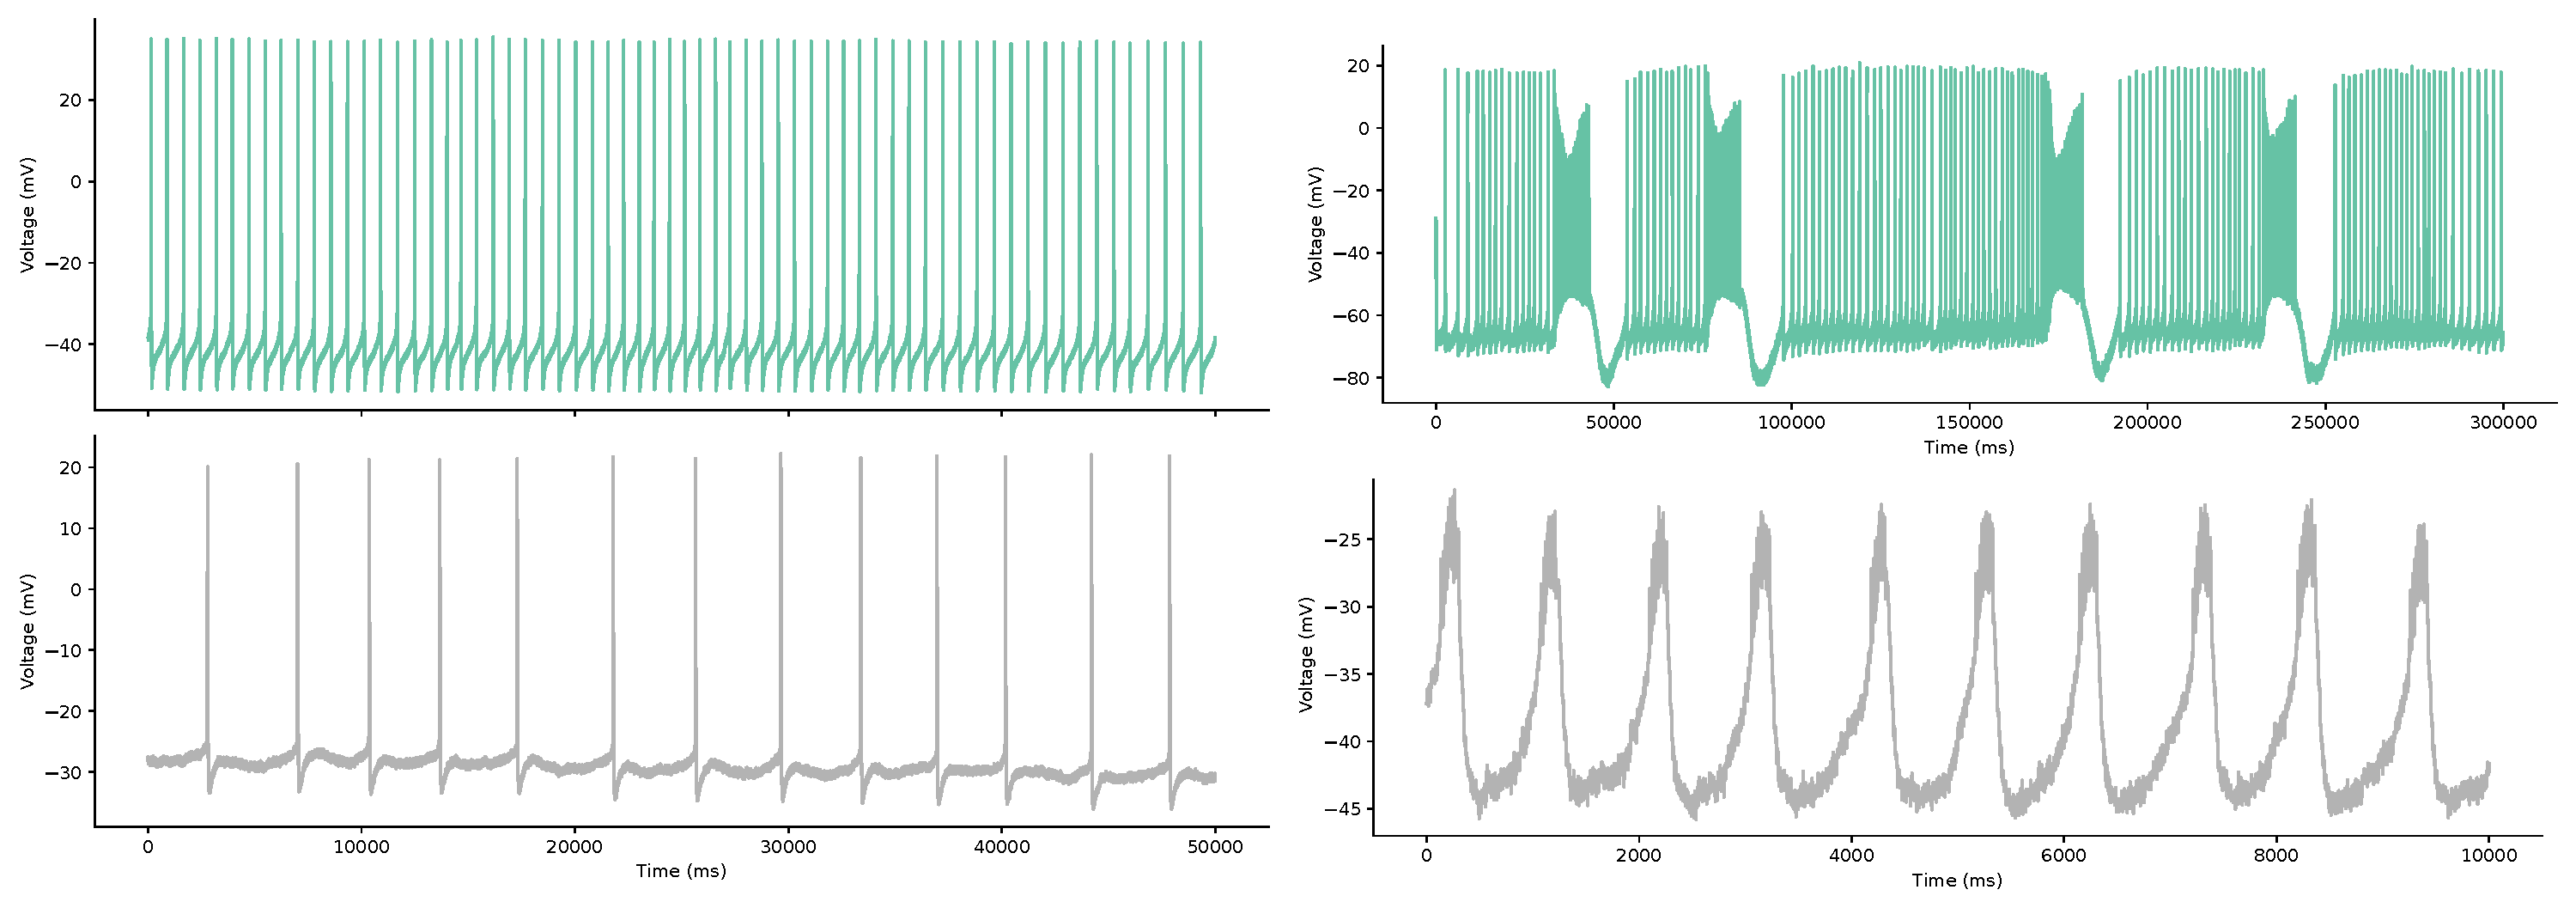
\includegraphics[width=0.7\textwidth]{intro/spike_activity-types.pdf}
	\end{center}}
\end{frame}

\begin{frame}{The sequential nature of neural dynamics}
	 \begin{columns}
			\begin{column}{0.6\textwidth}
				\begin{itemize}
					\item<1->{There are sequential processes at different time-scales.} 
					\item<3->{Many behaviors and actions are governed by sequential processes}
					\item<4->{Motor control, speech, decision making, etc. }
%					\item<5->{Studying sequential activity at different scales is crucial for a complete comprehension of neural systems.}
					\item<5->{Sequential dynamical invariants might have a crucial role in neural coordination to autonomously establish a balance between the robustness and flexibility required for effective function.}
				\end{itemize}
			\end{column}
			\begin{column}{0.45\textwidth}
				\uncover<2->{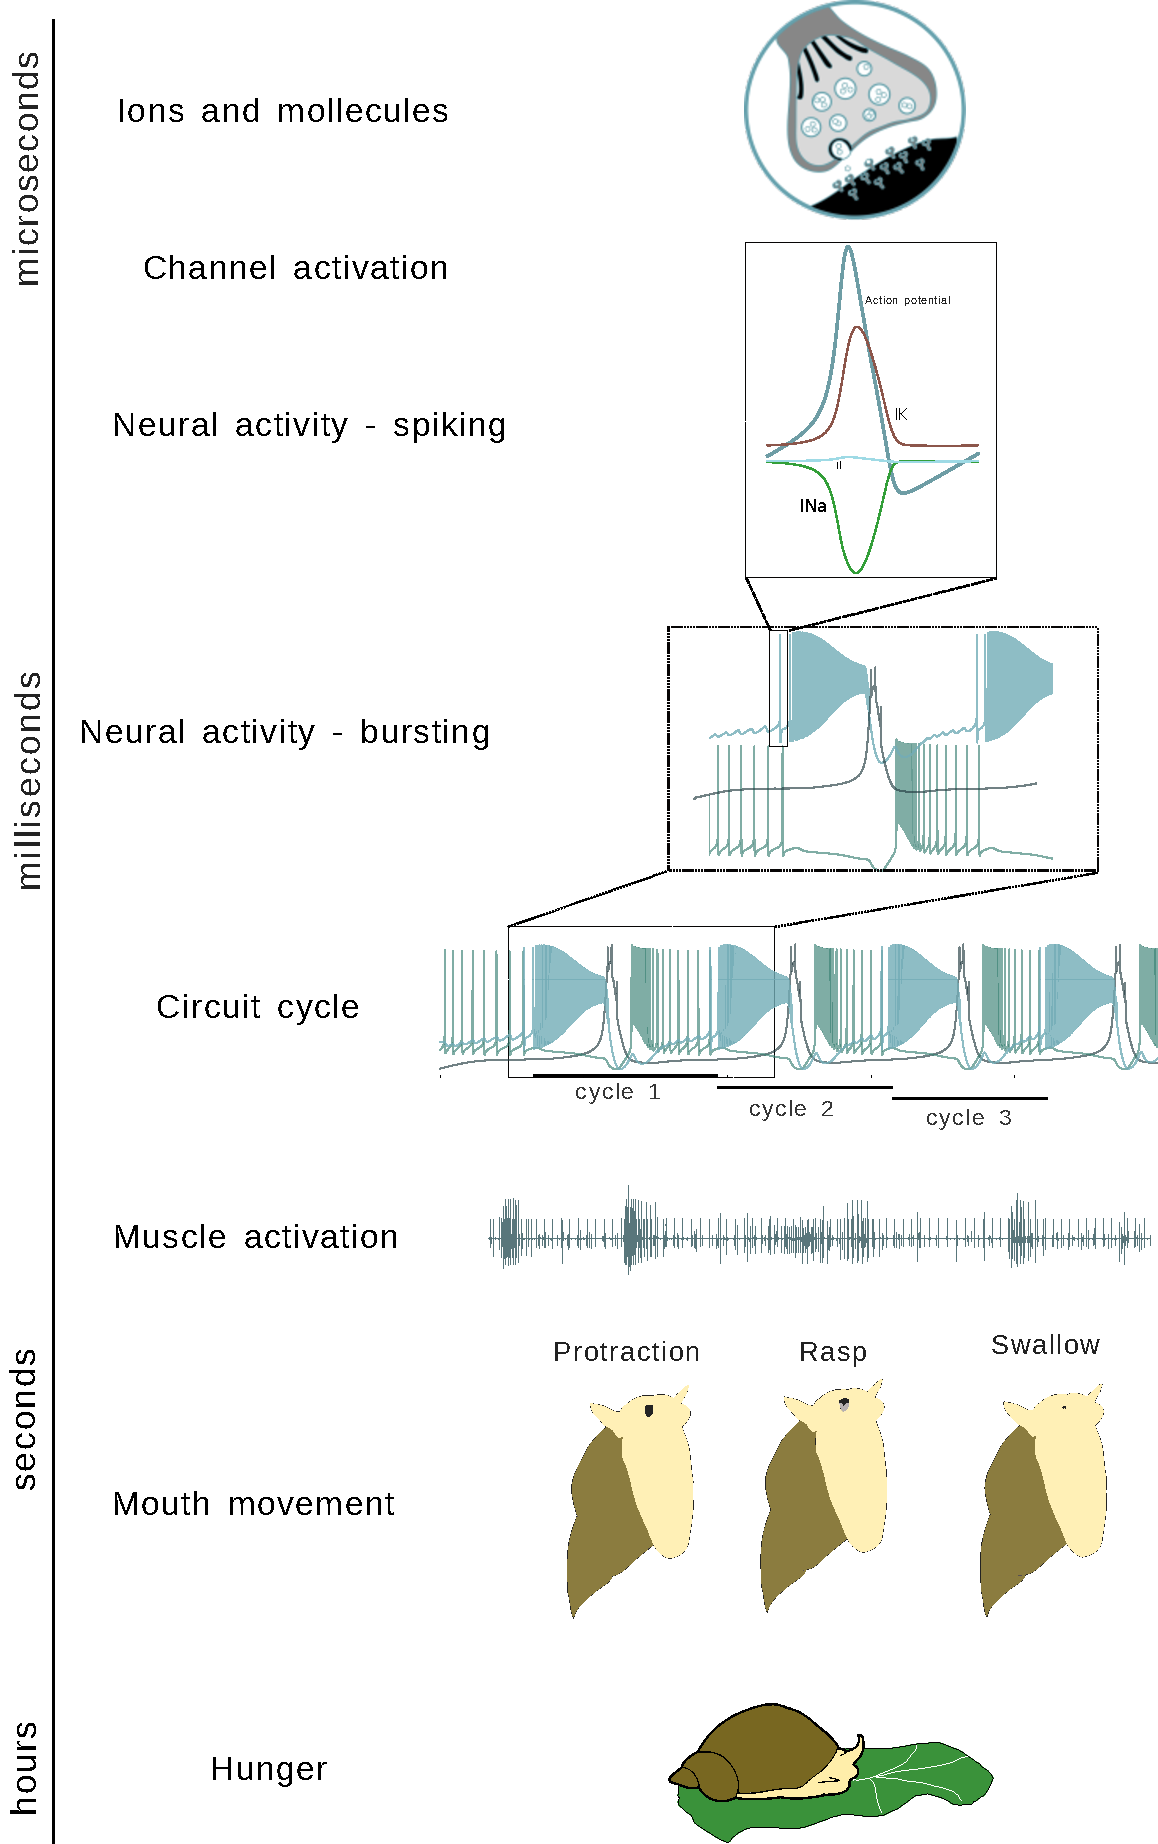
\includegraphics[width=\textwidth]{intro/time scale/time-scale-feeding.pdf}}
			\end{column}
		\end{columns}
	 
\end{frame}
\begin{frame}{Studying neural dynamics in computational models}
	\only<1-8>{
		\begin{itemize}
			\item<1-8>{Computational models are powerful tools to study neural dynamics}
			\item<2-8>{Advantages}
			\begin{itemize}
				\item<3-8>Full accessibility to the system
				\item<4-8>Detailed reproduction of the living activity
			\end{itemize}
			\item<5-8>{Limitations}
			\begin{itemize}
				\item<6-8>{Restricted variability}
				\item<7-8>{The description may depend on the information about the living system}
			\end{itemize}
		\end{itemize}
	}
	
	\only<10-11>{
		\textbf{Conductance-based models}
		\uncover<11>{\begin{table}[h!]
			\resizebox{\textwidth}{!}{%
				\begin{tabular}{lccc}
					Voltage equation                                                                 & \multicolumn{3}{c}{$C \frac{dV}{dt} = I - g_K n^4 (V - E_K) - g_{Na} m^3h(V-E_{Na}) - g_L (V-E_L)$}                                                                                                                                  \\ \hline
					& \multicolumn{2}{c}{Activation variables}                                                                                                                              & Inactivation variable                                        \\ \hline
					\multicolumn{1}{c|}{\begin{tabular}[c]{@{}c@{}}gating \\ variables\end{tabular}} & \multicolumn{1}{c|}{$\frac{dm(t)}{dt}=\frac{m_{\infty}(V(t))-m(t)}{\tau_m(V(t))}$} & \multicolumn{1}{c|}{$\frac{dn(t)}{dt}=\frac{n_{\infty}(V(t))-n(t)}{\tau_n(V(t))}$} & $\frac{dh(t)}{dt}=\frac{h_{\infty}(V(t))-h(t)}{\tau_h(V(t))}$ \\ \hline
				\end{tabular}%
			}
		\end{table}
	}
	}


	\only<12-13>{
	\textbf{Conductance-based models}
	\\
	\uncover<12->{By \textbf{different combinations of ionic channels} we can achieve \textbf{different activities and waveform shapes}}
	\uncover<13>{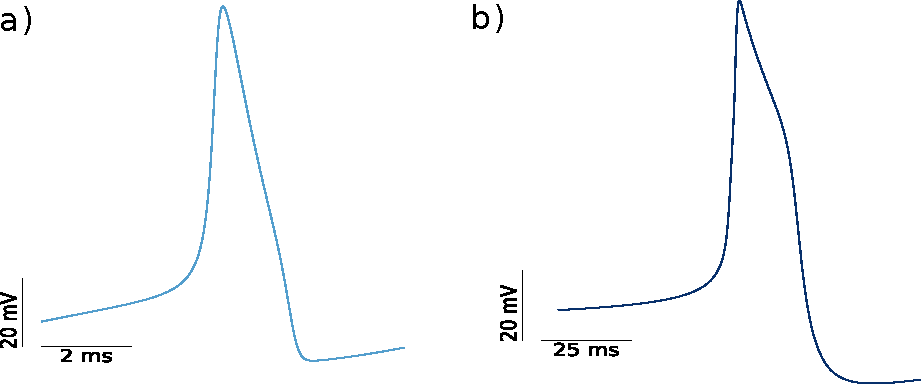
\includegraphics[width=\linewidth]{intro/spike-types model.pdf}}
	}

\only<14-15>{
	\textbf{Conductace-based models\\}
	\uncover<14->{By \textbf{modeling synapses} we can model whole \textbf{circuits} by connecting single modeled neurons.\\}
	\uncover<15>{\centering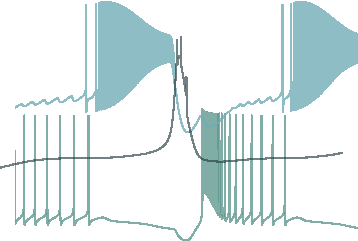
\includegraphics[width=0.7\linewidth]{intro/cpg.pdf}}
}
\end{frame}


\begin{frame}{Vertebrate and invertebrate animal studies}
	\only<1-7>{
	\begin{itemize}
	\item<1->In addition to the well known vertebrate models, there have been invaluable findings using invertebrates.
	\item<2->There are many universal characteristics of nervous systems and behaviors that can be extrapolated to humans.
	\item<3->Using invertebrates as animal models have different advantages:
		\begin{itemize}
			\item<4->Ease of accessibility to the nervous system.
			\item<5-> Longer survival times of the preparations.
			\item<6-> Ease of breeding and reproduction. 
			\item<7-> Full description of their systems. 
		\end{itemize}
	\end{itemize}
}
	\only<8->{
		\begin{columns}[t]
			\column{0.4\textwidth}
			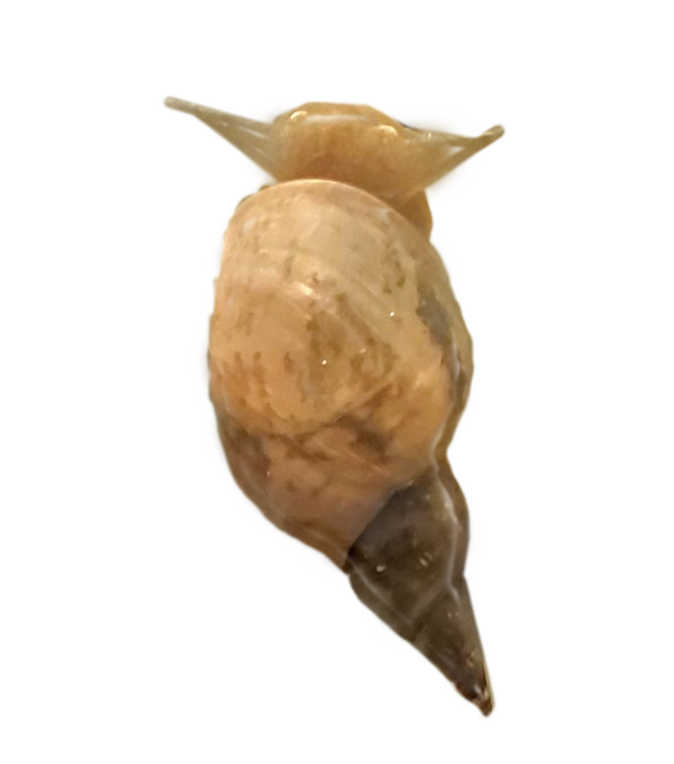
\includegraphics[width=\linewidth]{intro/lymnaea.png}
			
			\column{0.6\textwidth}
			\vspace{-4cm} % Adjust this value to align the text as needed
			\begin{itemize}
				\item<8->In this thesis we work with the neural system of \textit{Lymanea stagnalis}.
				\item<9>A pond snail whose system is well studied and described.
			\end{itemize}
		\end{columns}
	}
\end{frame}

\begin{frame}{Neural stimulation}
	\only<1-3>{
	When studying neural systems, we need neuromodulatory technics.
	\begin{itemize}
		\item <1-> To study different conditions.
		\item <2-> Test their robustness.
		\item <3-> Simulate external inputs.
	\end{itemize}
	}
	\only<4->{We can classify them based on: 
	\begin{itemize}
		\item<5-> The change in the system: Invasive / \textcolor<13>{red}{non-invasive}
		\item<6-> The source of the stimulation: 
			\begin{itemize}
				\item<7->{Chemical}
				\item<8->\textcolor<12>{red}{Electrical}
				\item<9->{Magnetic}
				\item<10->{Mechanical}
				\item<11->\textcolor<13>{red}{Optical}			
			\end{itemize}
	\end{itemize}	
}
		
\end{frame}

\section{Motivation and Objectives}
\begin{frame}{Motivation and Objectives}
	\begin{enumerate}
		\only<1-6>{
			\item<1-> To explore the \textbf{sequential nature of neuronal dynamics} at distinct description levels.
			\item<2-> To study \textbf{sequence interval variability} constraints and relationships in neural models and living circuits.
			\item<3-> To analyze the feeding CPG of \textit{Lymnaea stagnalis} to provide evidence of the\textbf{ universality of sequential dynamical invariants} found in the pyloric CPG by:
			\begin{enumerate}
				\item<4-> Characterizing the sequential invariants cycle-by-cycle in a bursting CPG model.
				\item<5-> Analyzing intracellular recordings with spontaneous activity and with different rhythm initiation stimulation protocols.
			\end{enumerate}
			\item<6-> To illustrate the possible \textbf{functionality} of sequential dynamical invariants in biohybrid robotics.
		}
		\only<7-11>{
			\setcounter{enumi}{4}
			\item<7-> To test the capability of \textbf{CW-NIR laser stimulation to modulate} neuronal dynamics by:
			\begin{enumerate}
				\item<8-> Characterizing the CW-NIR effect in the spike waveform dynamics.
				\item<9-> Analyzing the ability of this neurotechnology to change the spiking rate and the circuit dynamics.
			\end{enumerate}
			\item<10-> To study the possible \textbf{biophysical candidates} underlying the CW-NIR effect in model simulations.
			\item<11-> To design and implement a \textbf{new technique} for CW-NIR stimulation in \textbf{closed-loop}.
		}
	\end{enumerate}
	
\end{frame}


\section[Sequential Dynamical Invariants]{Sequential constrains in CPG circuits:
	Dynamical invariants}

\begin{frame}{Central Pattern Generators}
	\only<1-4>{
		\begin{itemize}
			\item<1->{Neural circuits generating robust sequences of neural activity}
			\item<2->{Control motor rhythms in an autonomous manner}
			\item<3->{Present in vertebrates and invertebrates}
			\item<4->{Flexible enough to adapt the rhythm to the variability keeping a robust sequential activity}
		\end{itemize}
		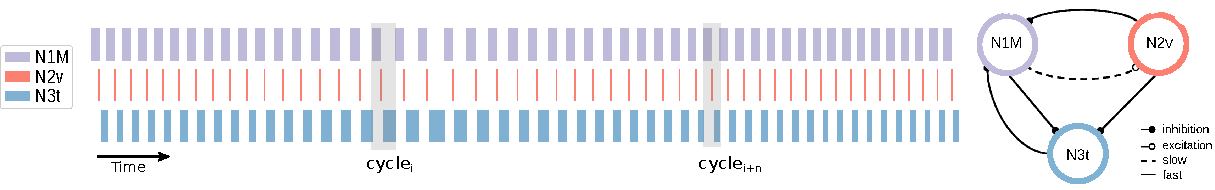
\includegraphics[width=\textwidth]{invariants/variability/sequences_in_cpgs.pdf}
	}
	\only<5->{
		\begin{columns}
			% First column in the first row
			\begin{column}{0.75\textwidth}
				\begin{itemize}
					\item<5->{Non-open topologies}
					\item<6->{Based on mutual inhibition}
					\item<7->{Temporal sequences maintained cycle-by-cycle}
				\end{itemize}
			\end{column}
			% Second column in the first row
			\begin{column}{0.3\textwidth}
				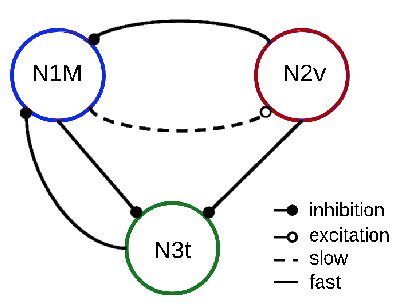
\includegraphics[width=\textwidth]{Images/CPG-topology.png} % Replace 'example-image' with your image file
			\end{column}
		\end{columns}
		
		% Second row
		\begin{figure}[h!]
			\centering
			\movie[label=CPG activity,width=0.7\textwidth,poster=false,autostart=false,showcontrols,loop] 
			{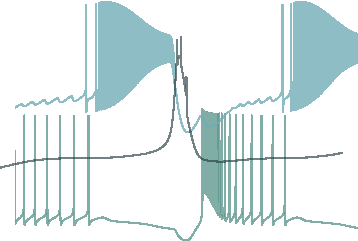
\includegraphics[width=0.7\textwidth]{intro/CPG.pdf}}{Movies/CPG_activity_slow.mp4}
		\end{figure}		
	}
\end{frame}

\begin{frame}{Temporal constrains: Sequential Dynamical invariants}
	\only<1-4>{
		\begin{itemize}
			\item<1->Recently found in pyloric CPG (experimental study). (Elices et al.)
			\item<2->Specific intervals that build the sequence are highly correlated cycle-by-cycle.
			\item<3->Consistent under high variability induced situations (Ethanol).
		\end{itemize}}
	\begin{figure}[h!]
		\centering
		\movie[label=pyloric video,width=\textwidth,poster=false,autostart=true,showcontrols,loop] 
		{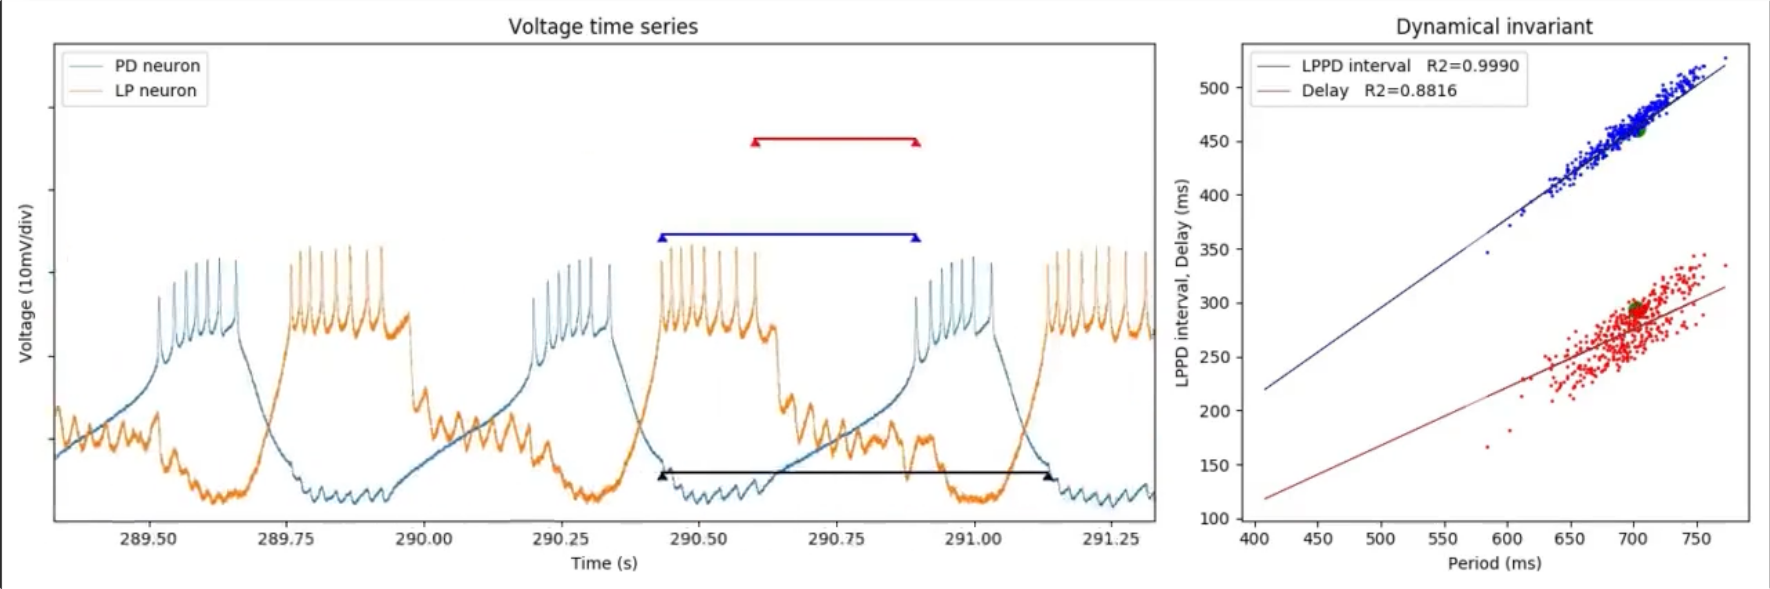
\includegraphics[width=\textwidth]{Movies/elices_invariants.png}}{Movies/elices_invariants.mp4}
	\end{figure}		
\end{frame}

\begin{frame}{Feeding CPG of \textit{Lymnaea stagnalis}}
		\begin{columns}
			% First column in the first row
			\begin{column}{0.45\textwidth}
				Triphasic rhythm:
				\begin{itemize}
					\item<1->{N1 phase $\rightarrow$ Protraction}
					\item<2->{N2 phase $\rightarrow$ Rasp}
					\item<3->{N3 phase $\rightarrow$ Swallow}
				\end{itemize}
			\end{column}
			% Second column in the first row
			\uncover<1->{
			\begin{column}{0.6\textwidth}
				\movie[label=cpg video,width=\textwidth,poster,autostart,borderwidth=-5pt,showcontrols,loop] 
				{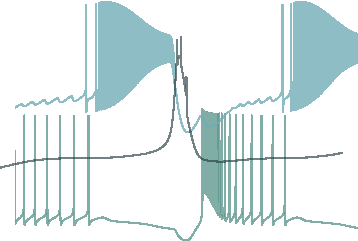
\includegraphics[width=\textwidth]{intro/cpg.pdf}}{Movies/CPG-lymnaea_v2_mejorado.mp4}
			\end{column}
		}
		\end{columns}
\end{frame}



\begin{frame}{Computational and Experimental approach}
	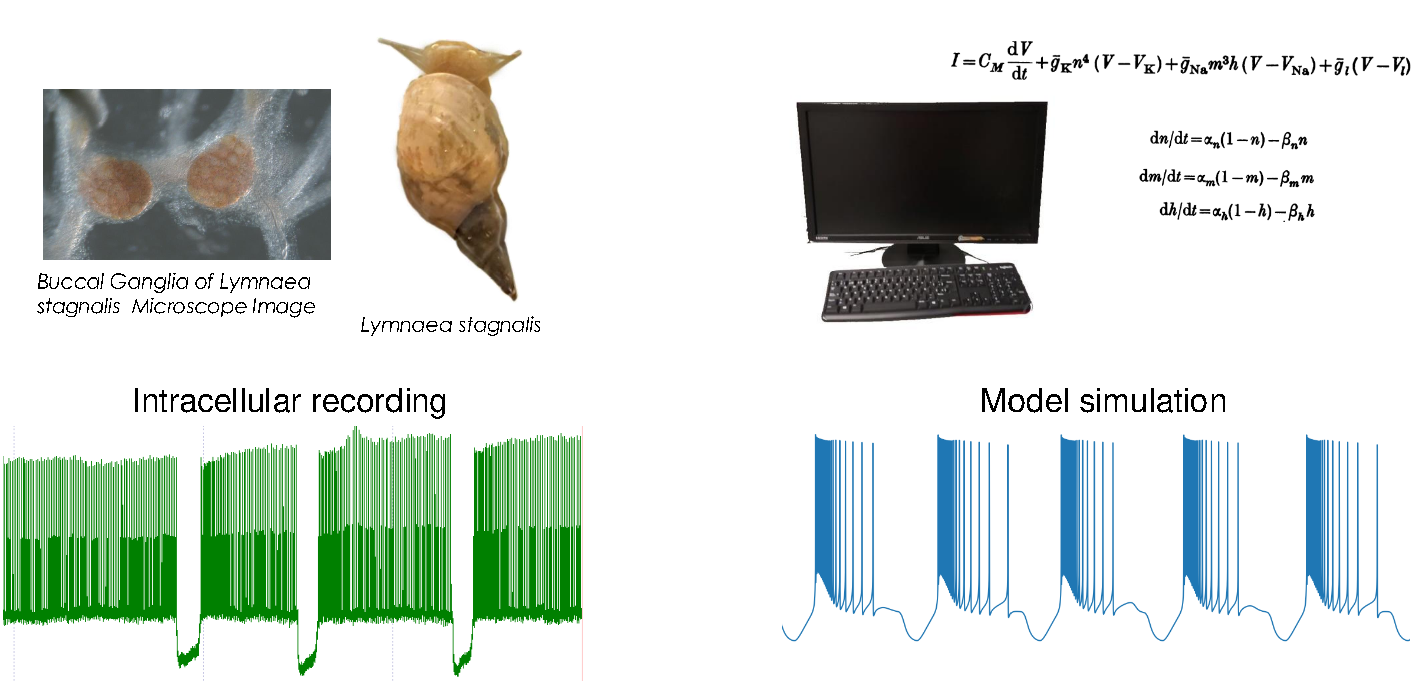
\includegraphics[width=\textwidth]{Images/experimental-computational.pdf})
\end{frame}




\begin{frame}{Charaterization of the time-intervals cycle-by-cycle}
	\begin{columns}
		\begin{column}{0.4\textwidth}
			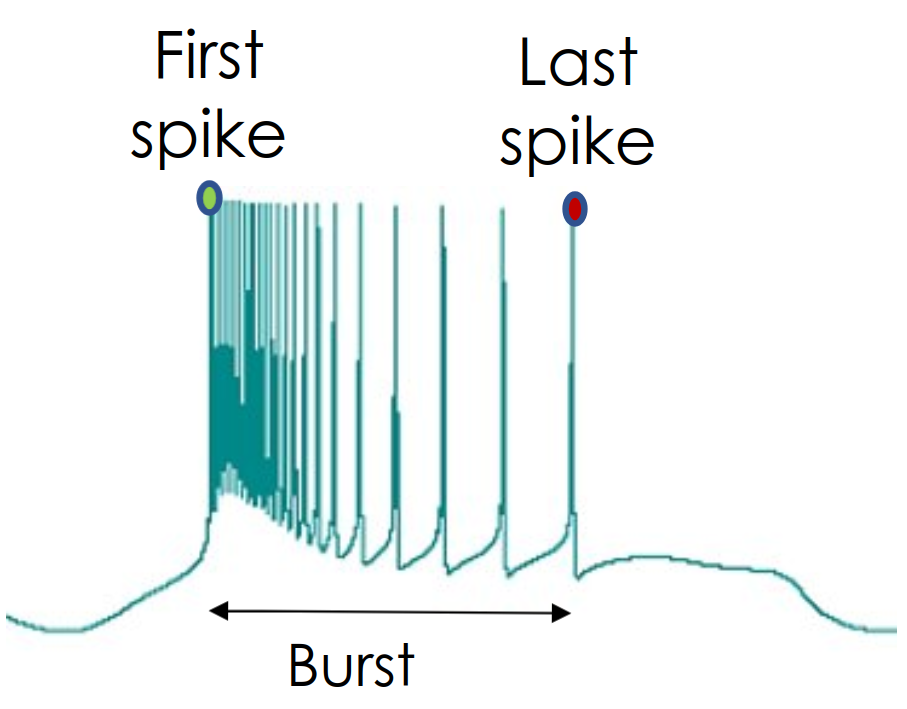
\includegraphics[width=\textwidth]{Images/time-references.png}
		\end{column}
		\begin{column}{0.6\textwidth}
			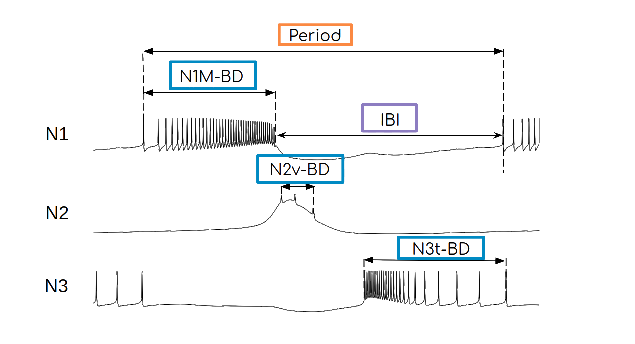
\includegraphics[width=\textwidth]{methods-paper-modelo/figure4a.eps}
		\end{column}
	\end{columns}
\end{frame}


\begin{frame}{Computational Approach: Model description}
	\begin{columns}
		\begin{column}{0.5\textwidth}
			\begin{itemize}
				\item<1->(Vavoulis et al.)
				\item<1->Conductance-based model.
				\item<1->Specific waveforms and gradual synapse.
				\item<1->Two compartments.
				\item<1->Feeding CPG Model.
			\end{itemize}
		\end{column}
		\begin{column}{0.5\textwidth}
			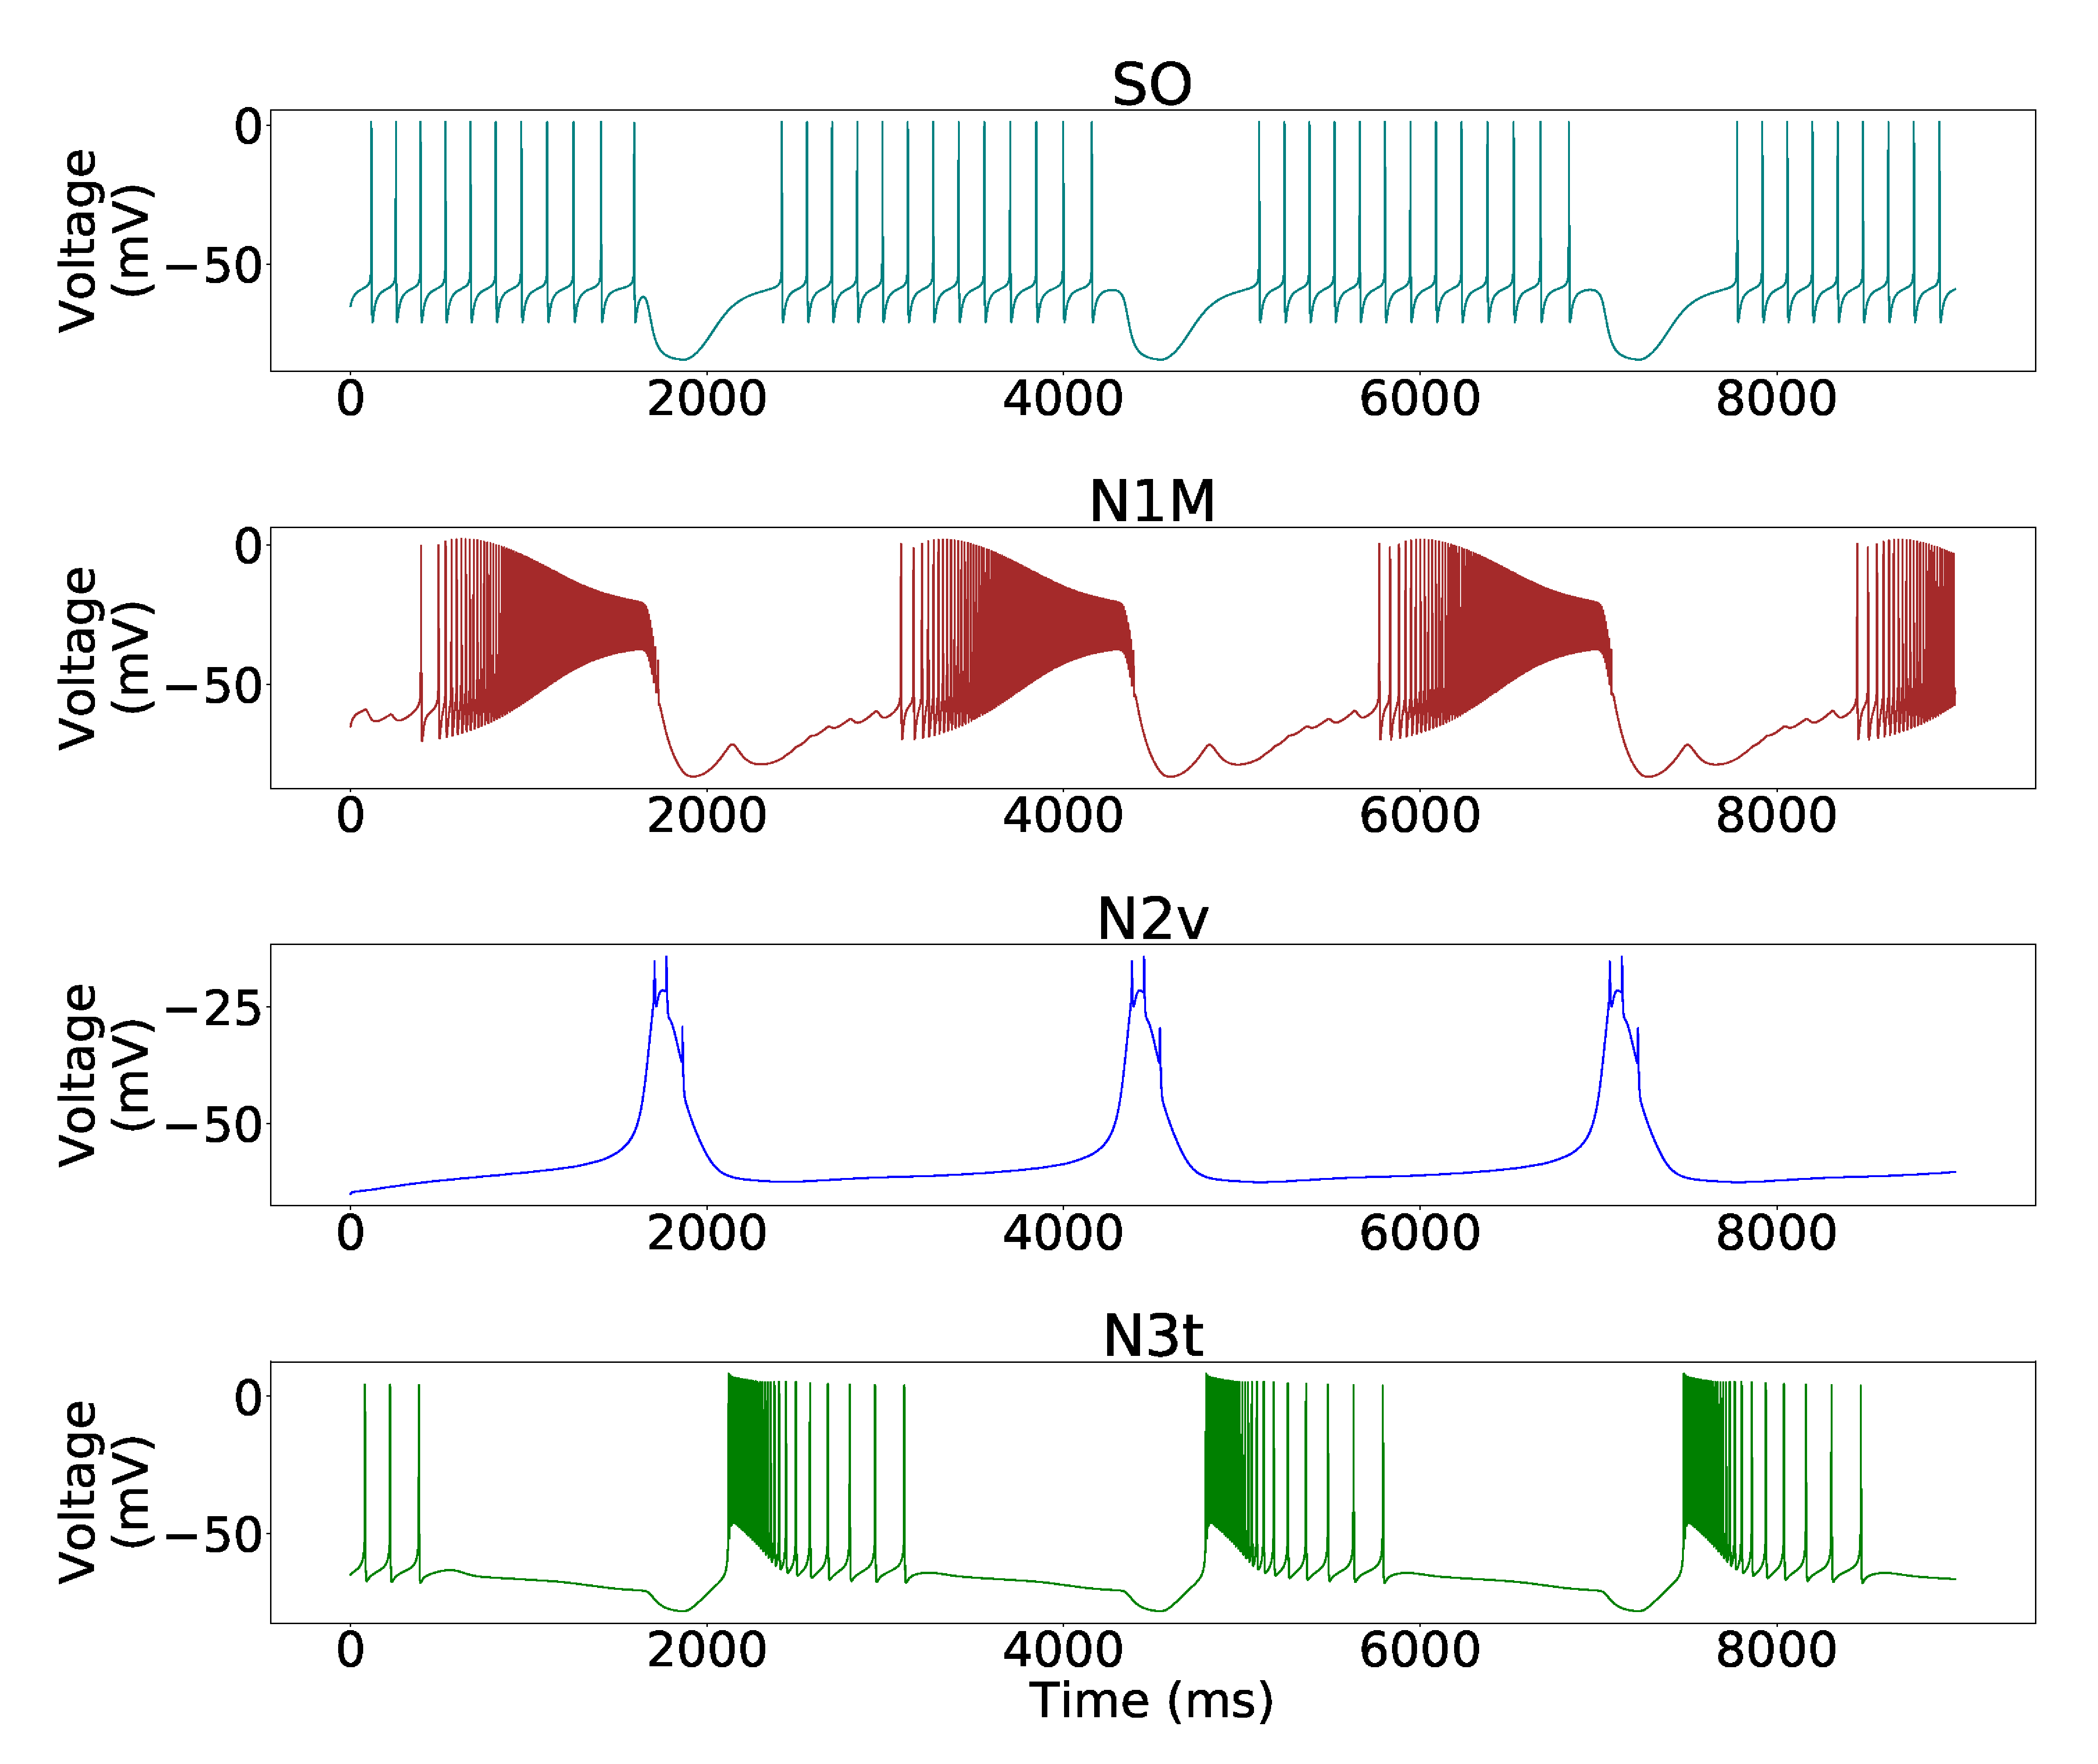
\includegraphics[width=\textwidth]{methods/invariants-model/figure2.eps}
		\end{column}
	\end{columns}
		\vspace{4pt}
		\centering
		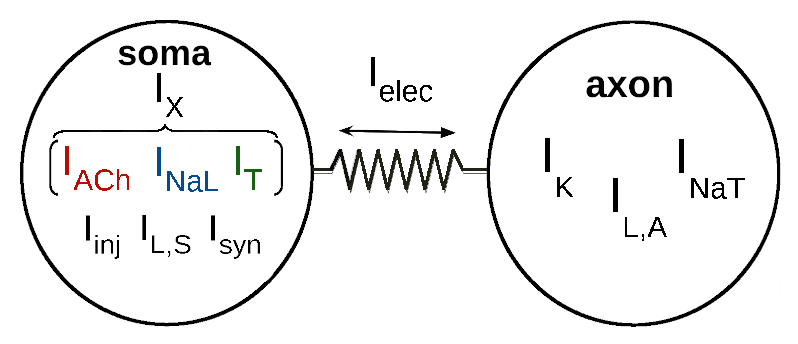
\includegraphics[width=0.6\textwidth]{methods/invariants-model/figure1a.eps}
\end{frame}



\begin{frame}{Computational Approach: Ramp stimulation protocol}
	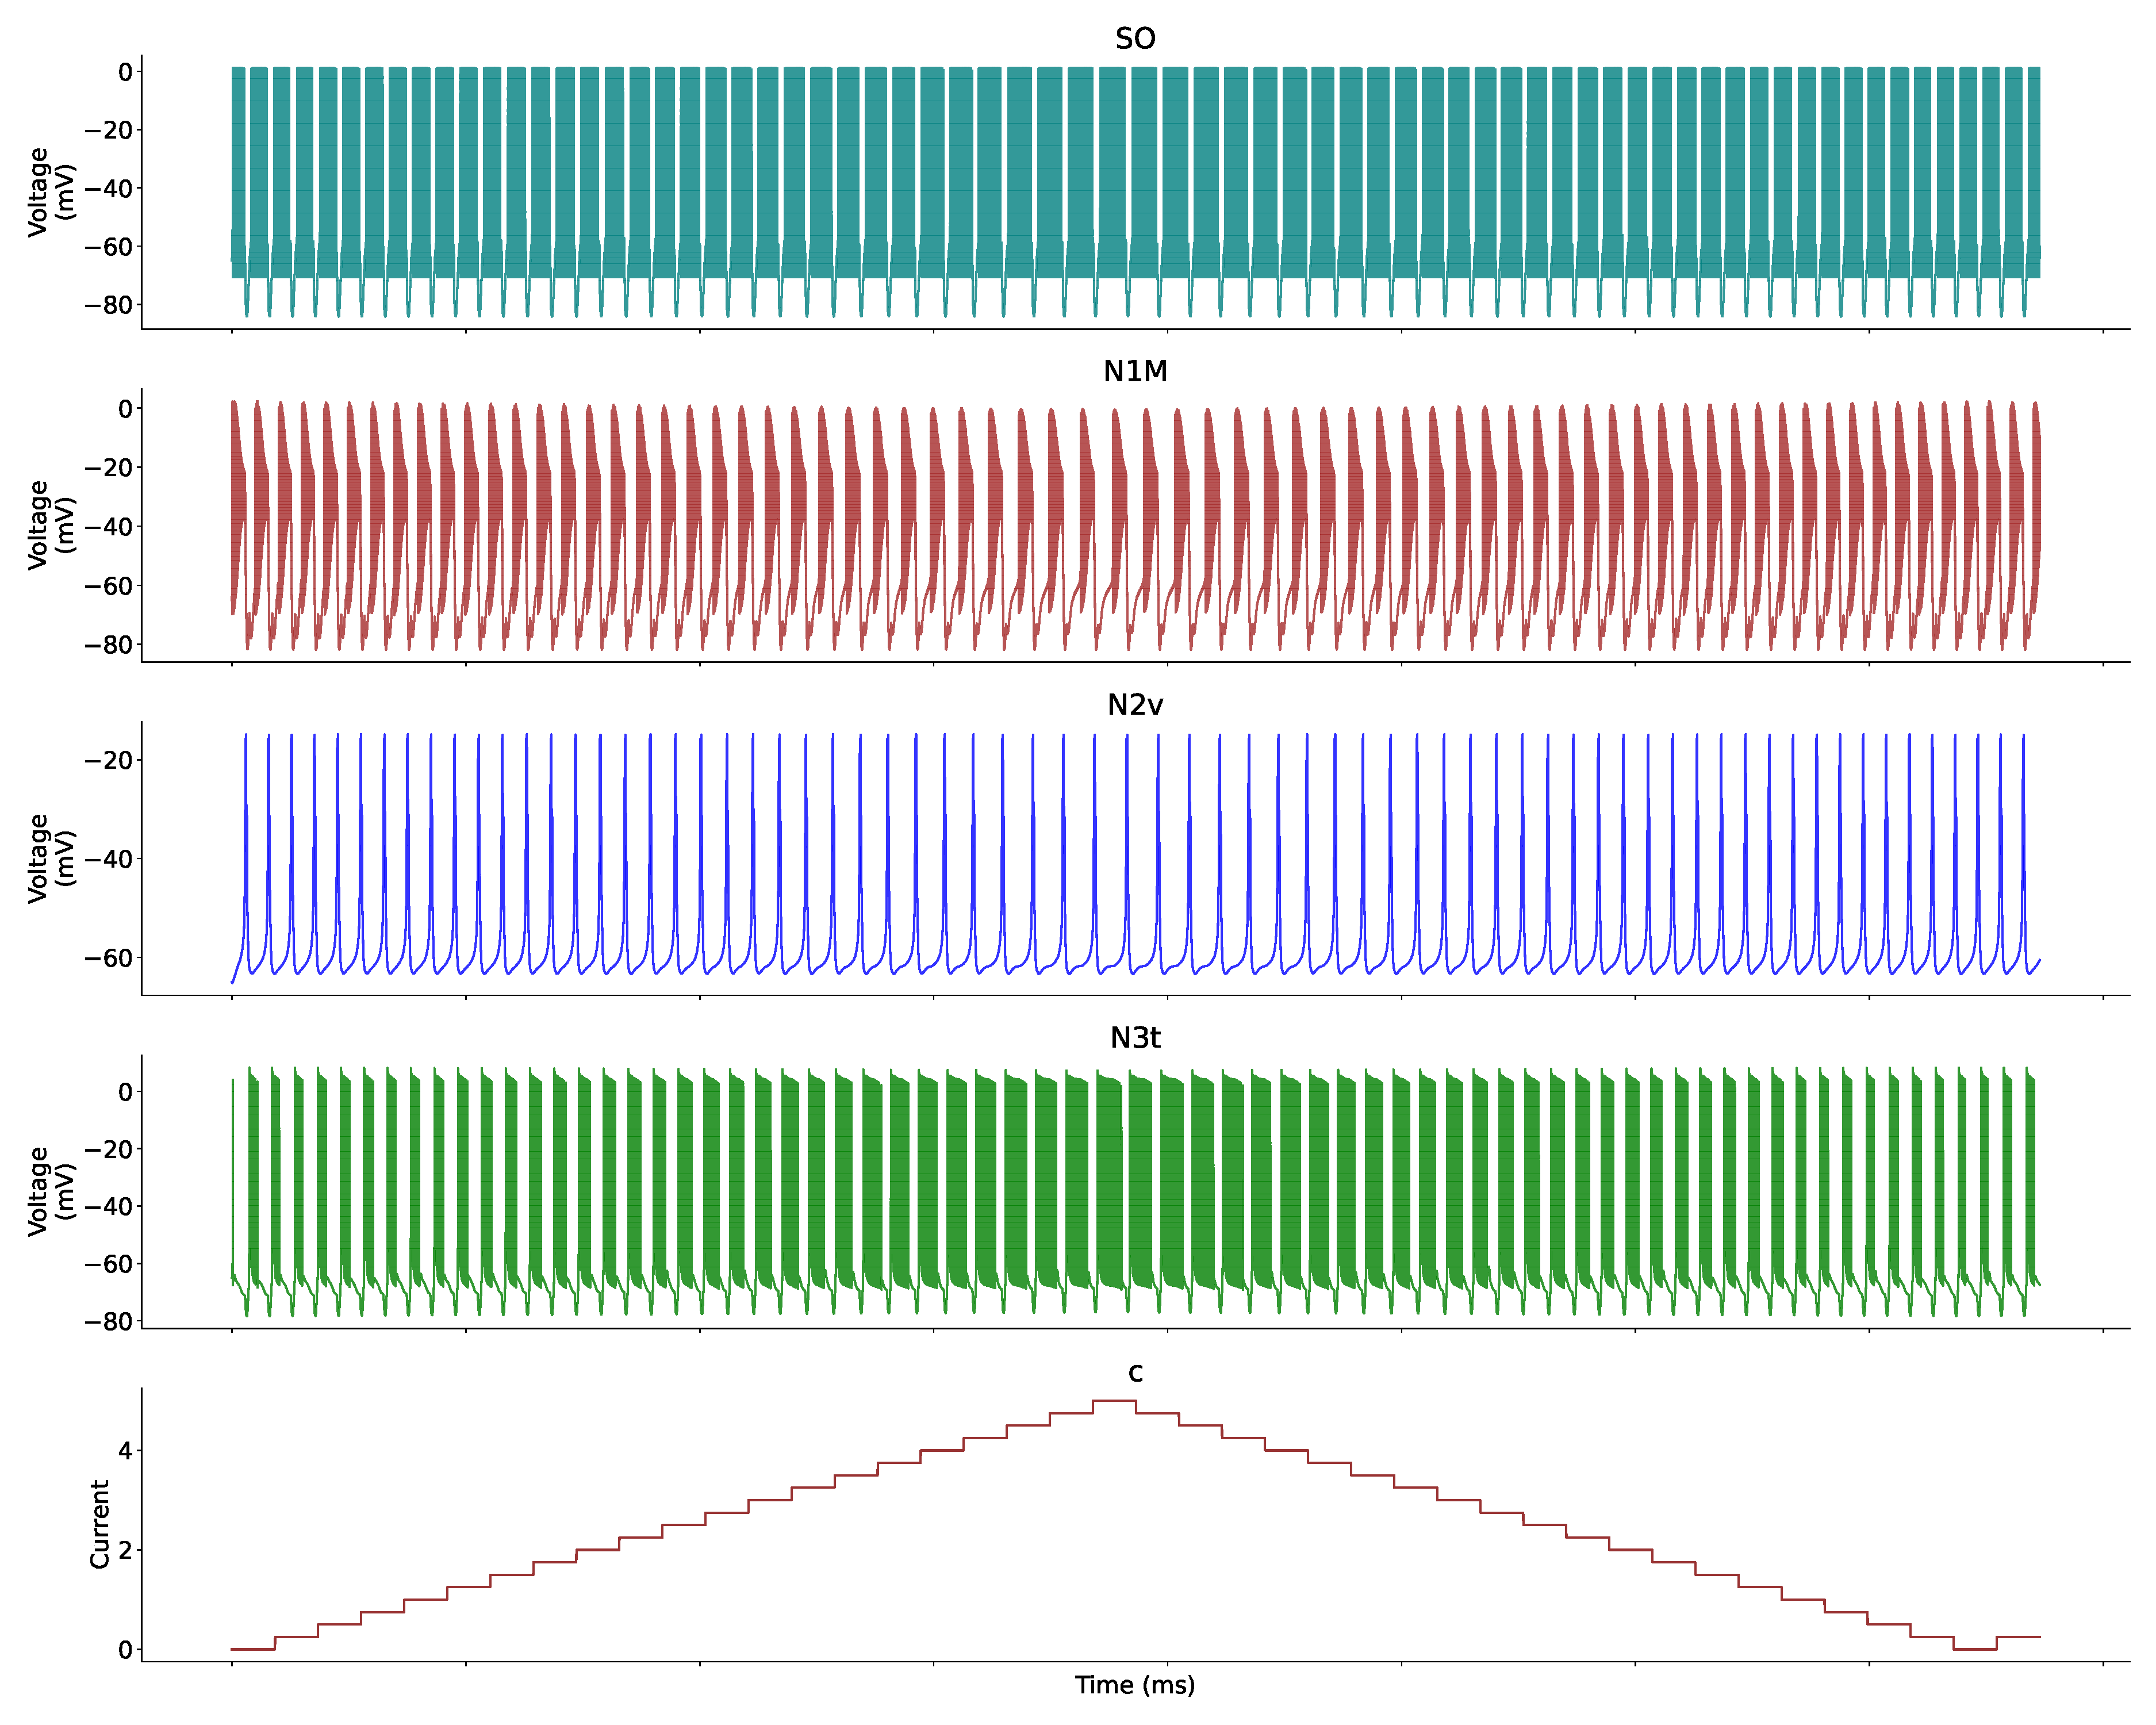
\includegraphics[width=\textwidth]{methods-paper-modelo/circuit_w_current.pdf}
\end{frame}

\begin{frame}{Cycle-by-cycle restrictions}
	\movie[label=model_invariants_video,width=\textwidth,poster,autostart,borderwidth=-5pt,showcontrols,loop] 
	{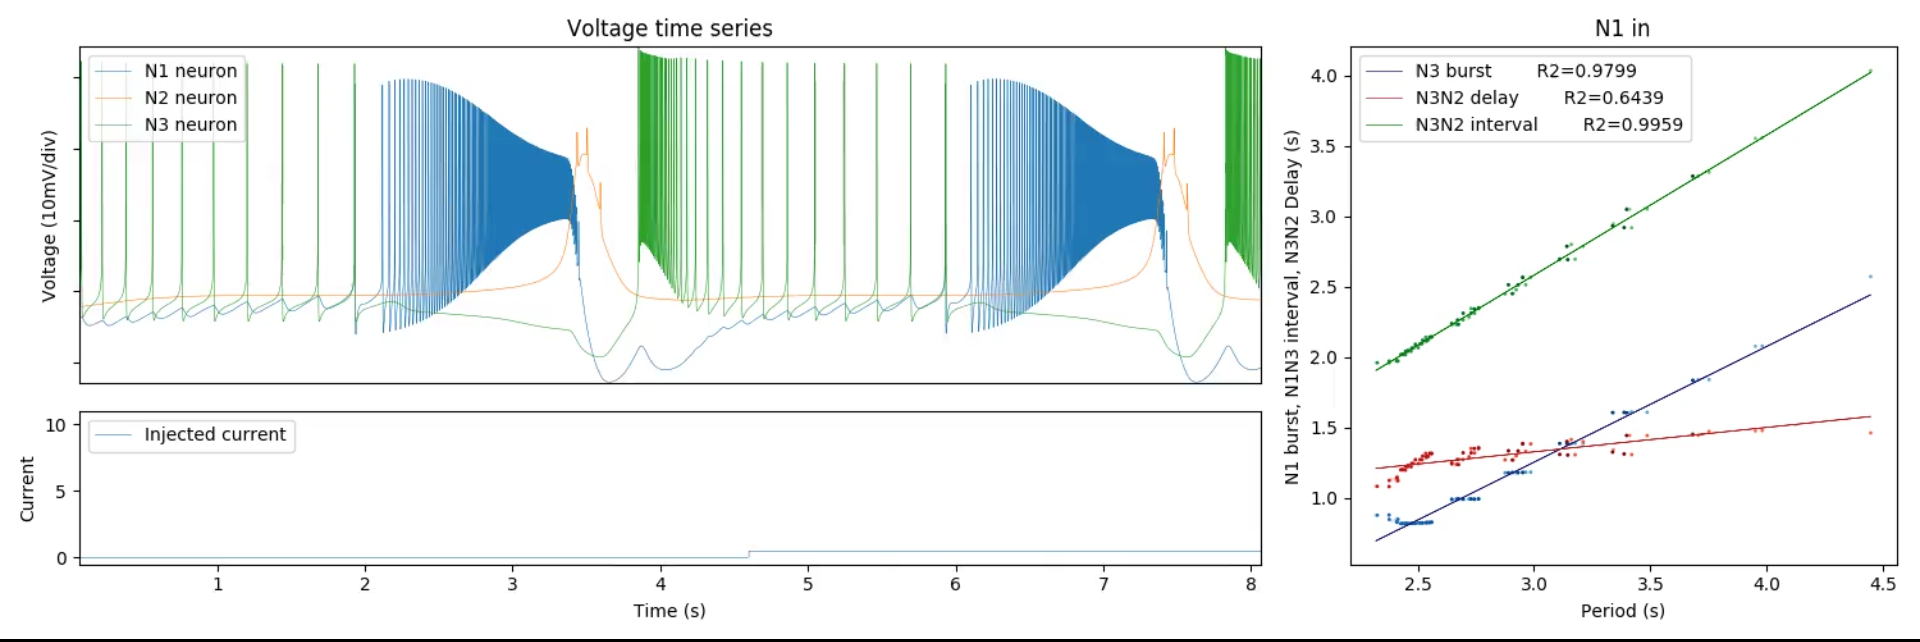
\includegraphics[width=\textwidth]{Movies/n3_n2_no_invariant.png}}{Movies/n3_n2_no_invariant.mp4}
\end{frame}

\begin{frame}{N1M stimulation}
	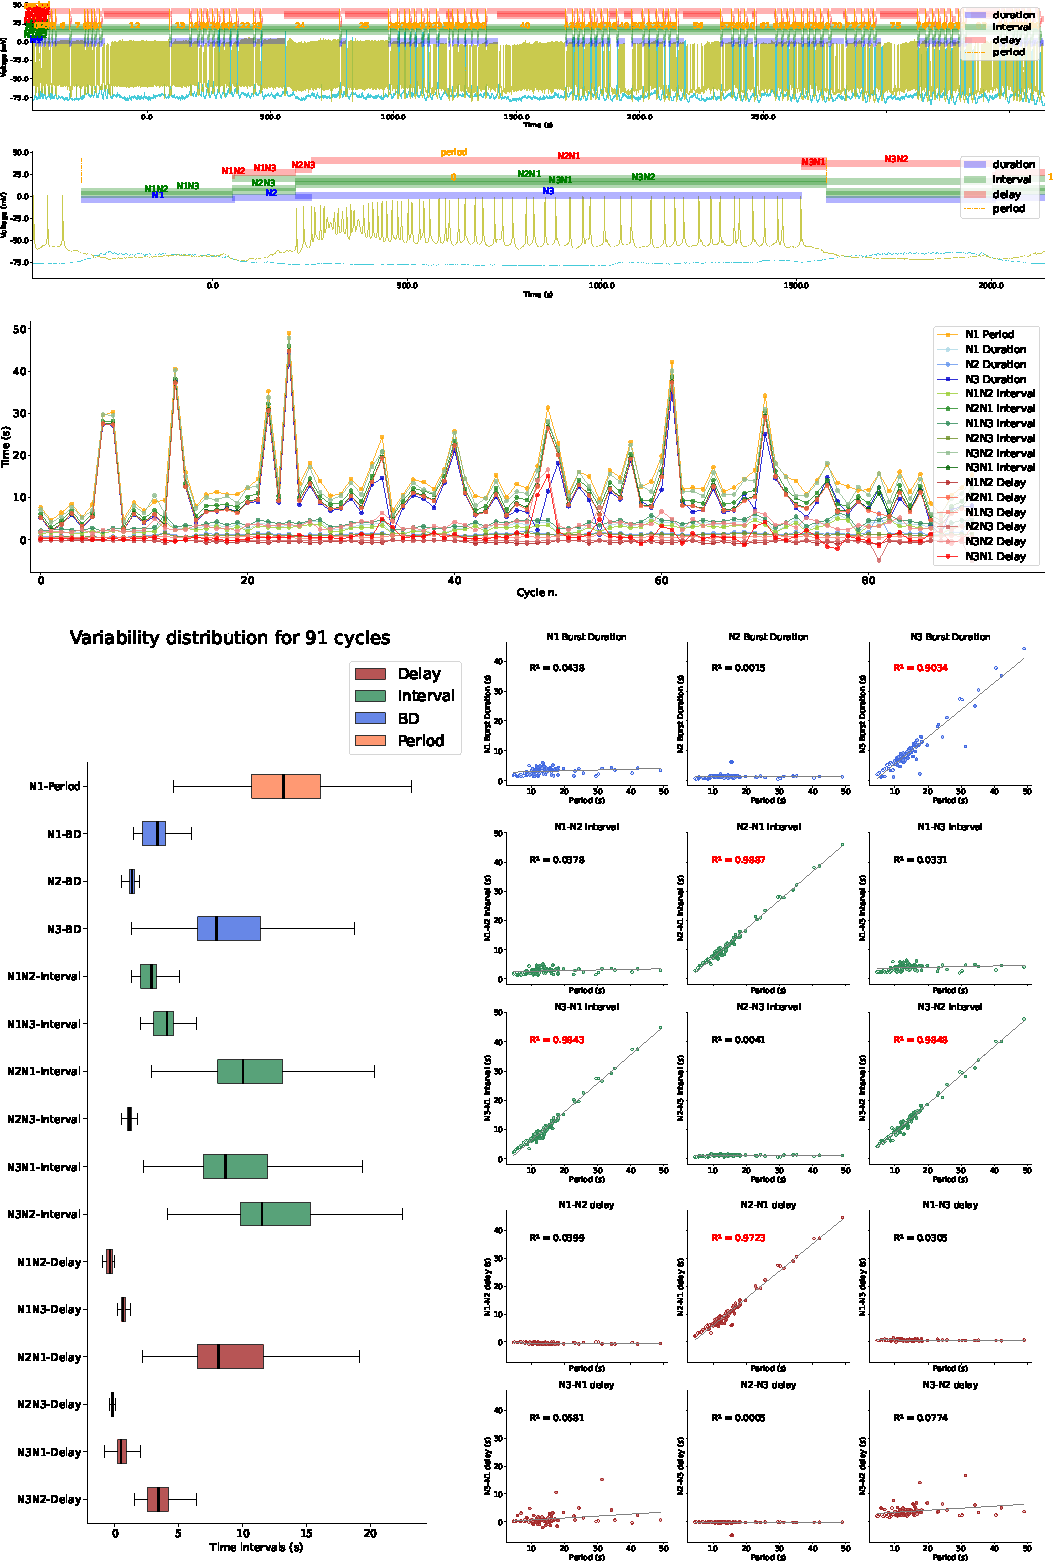
\includegraphics[width=\textwidth]{invariants/data/SUSSEX/prep2/images/3phases/panel_with_intervals.pdf}
	
\end{frame}


\begin{frame}{SO stimulation}
\end{frame}


\begin{frame}{Models with chaotic activity}
	Variability in models is usually limited. The variability can be induced by a current ramp as in this case, but with a chaotic activity the variability could be more realistic. 
	\vspace{8pt}
	\begin{columns}
		\uncover<2>{
			\begin{column}{0.5\textwidth}
				Neuronal recording variability
				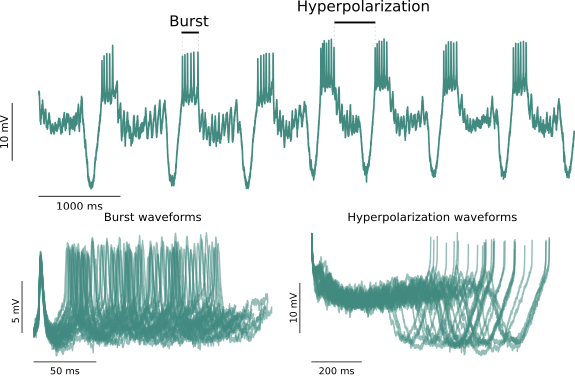
\includegraphics[width=\textwidth]{invariants/variability/lp_burst_variability.png}
			\end{column}
		}
		\uncover<3>{
			\begin{column}{0.5\textwidth}
				Model simulation with chaotic activity
				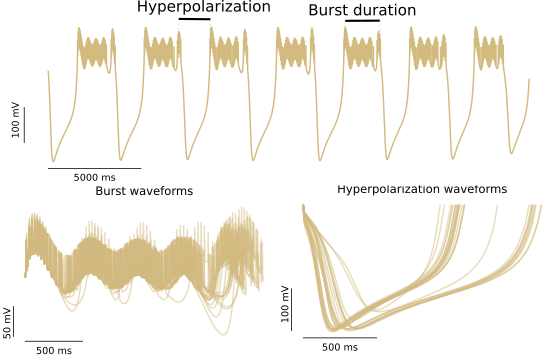
\includegraphics[width=\textwidth]{invariants/variability/TN-burst_variability.png}
			\end{column}
		}
	\end{columns}
\end{frame}



\begin{frame}{Experimental approach}
	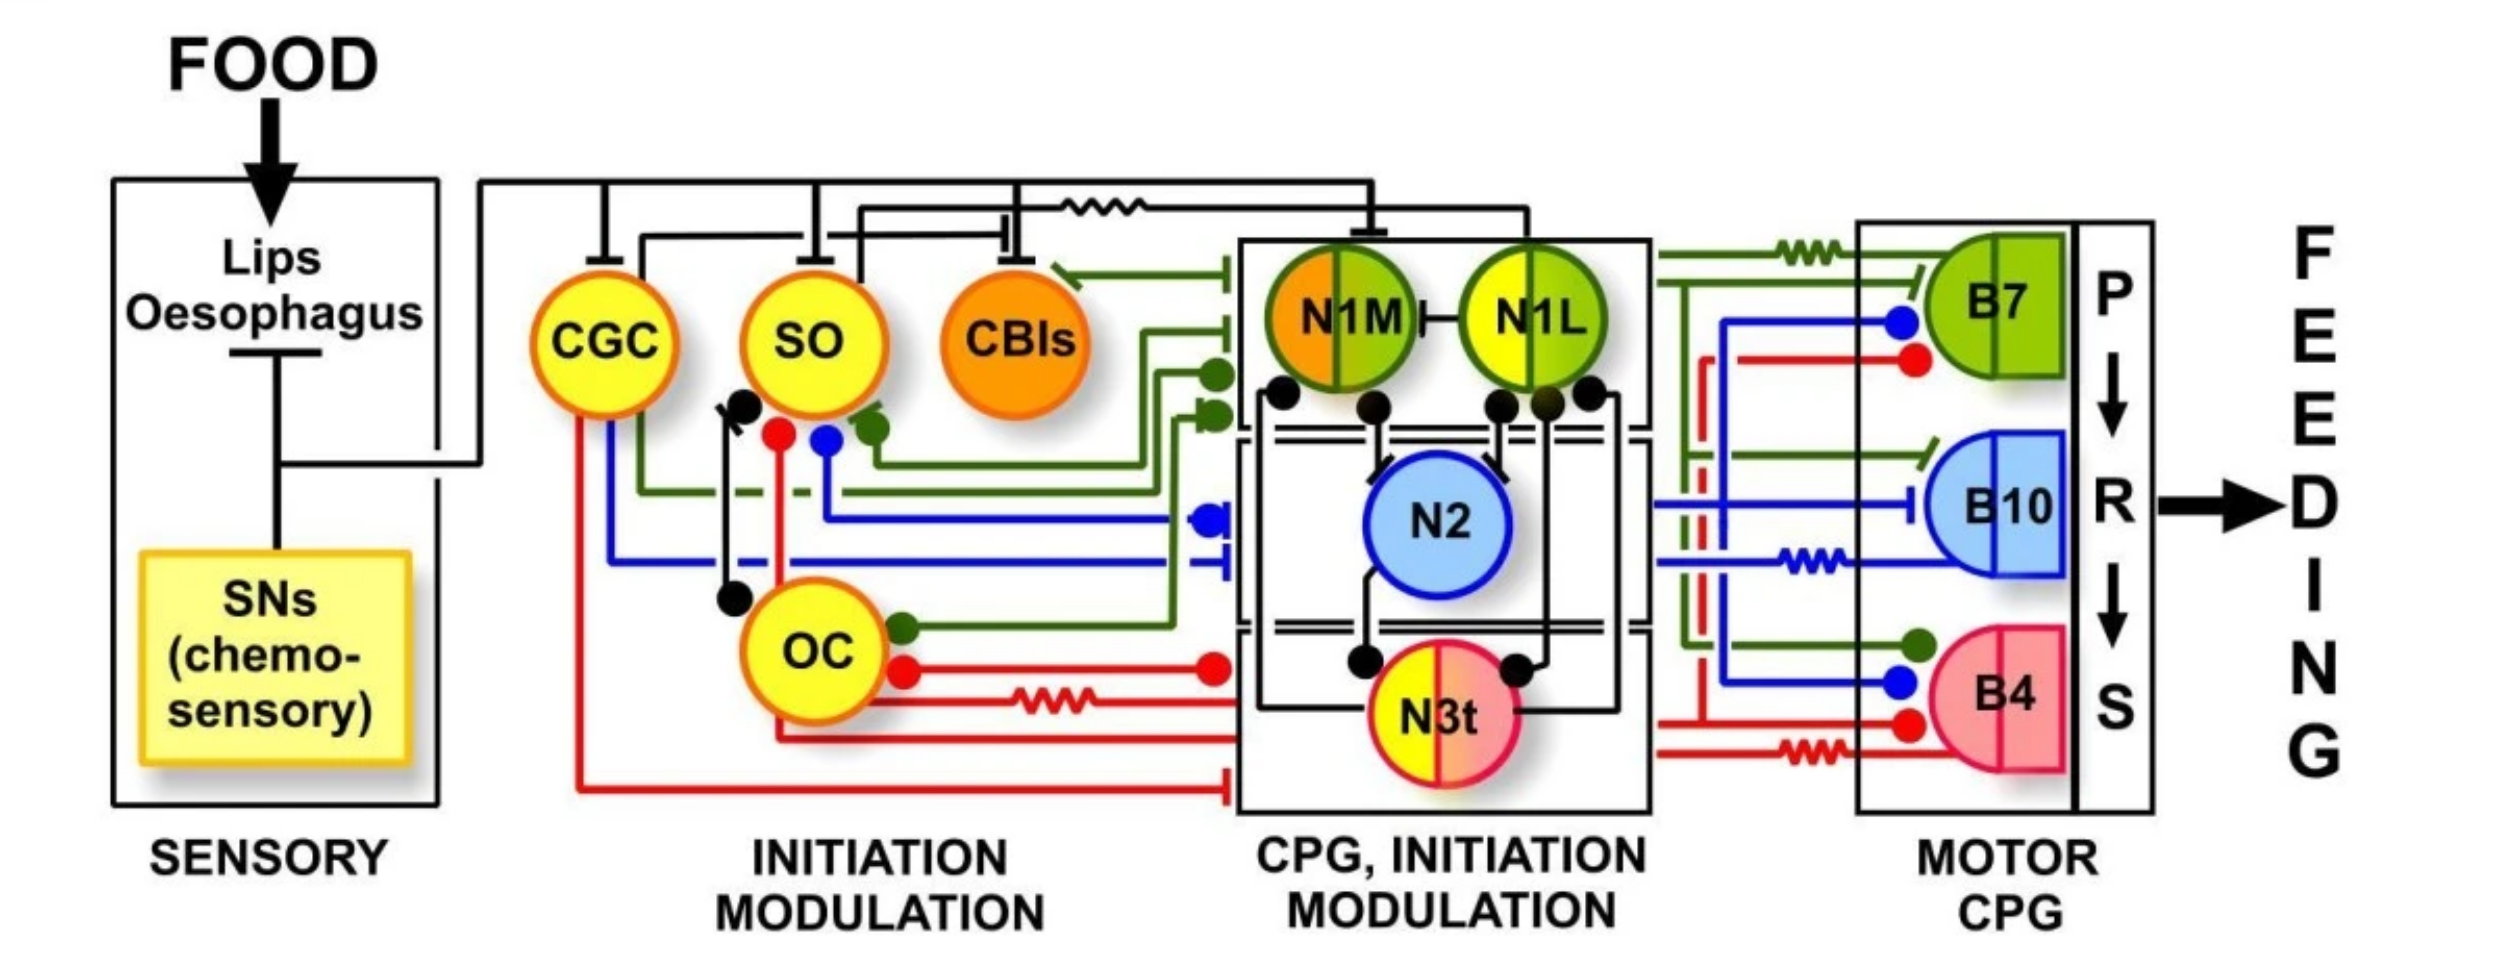
\includegraphics[width=\textwidth]{invariants/distributed_benjamin_2012.png}
\end{frame}



\begin{frame}{Spontaneous activity}
	\begin{columns}
		\begin{column}{0.5\textwidth}
			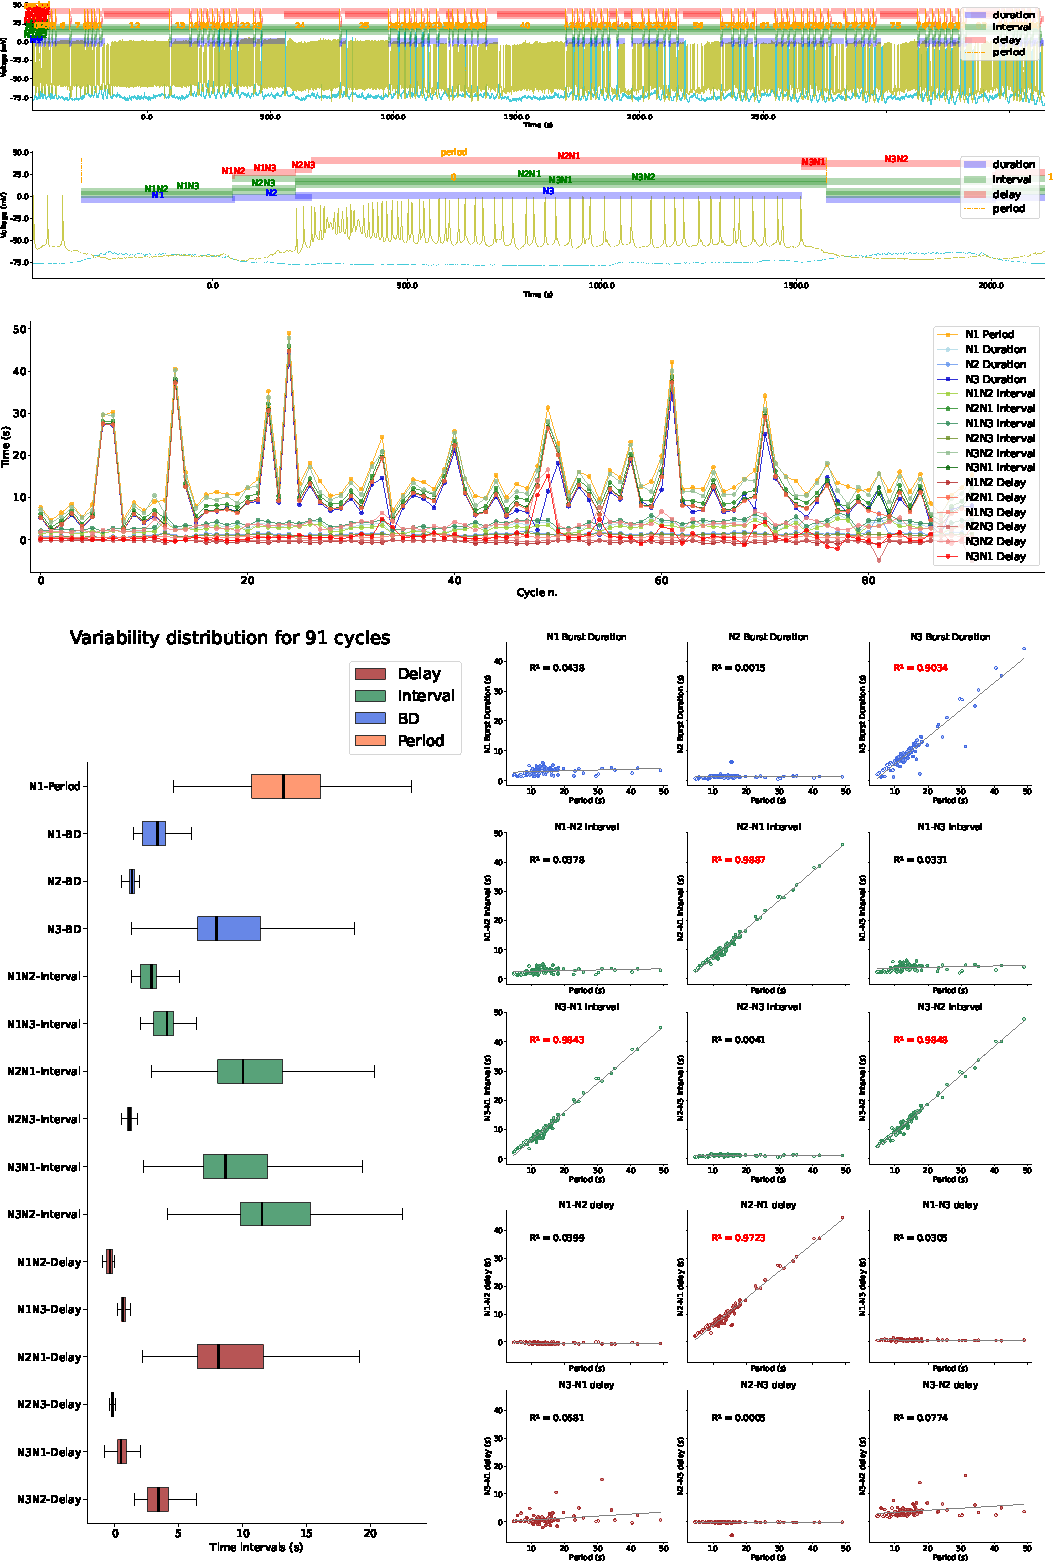
\includegraphics[width=\textwidth]{invariants/data/SUSSEX/prep2/images/3phases/panel_with_intervals.pdf}
		\end{column}
		\begin{column}{0.5\textwidth}
			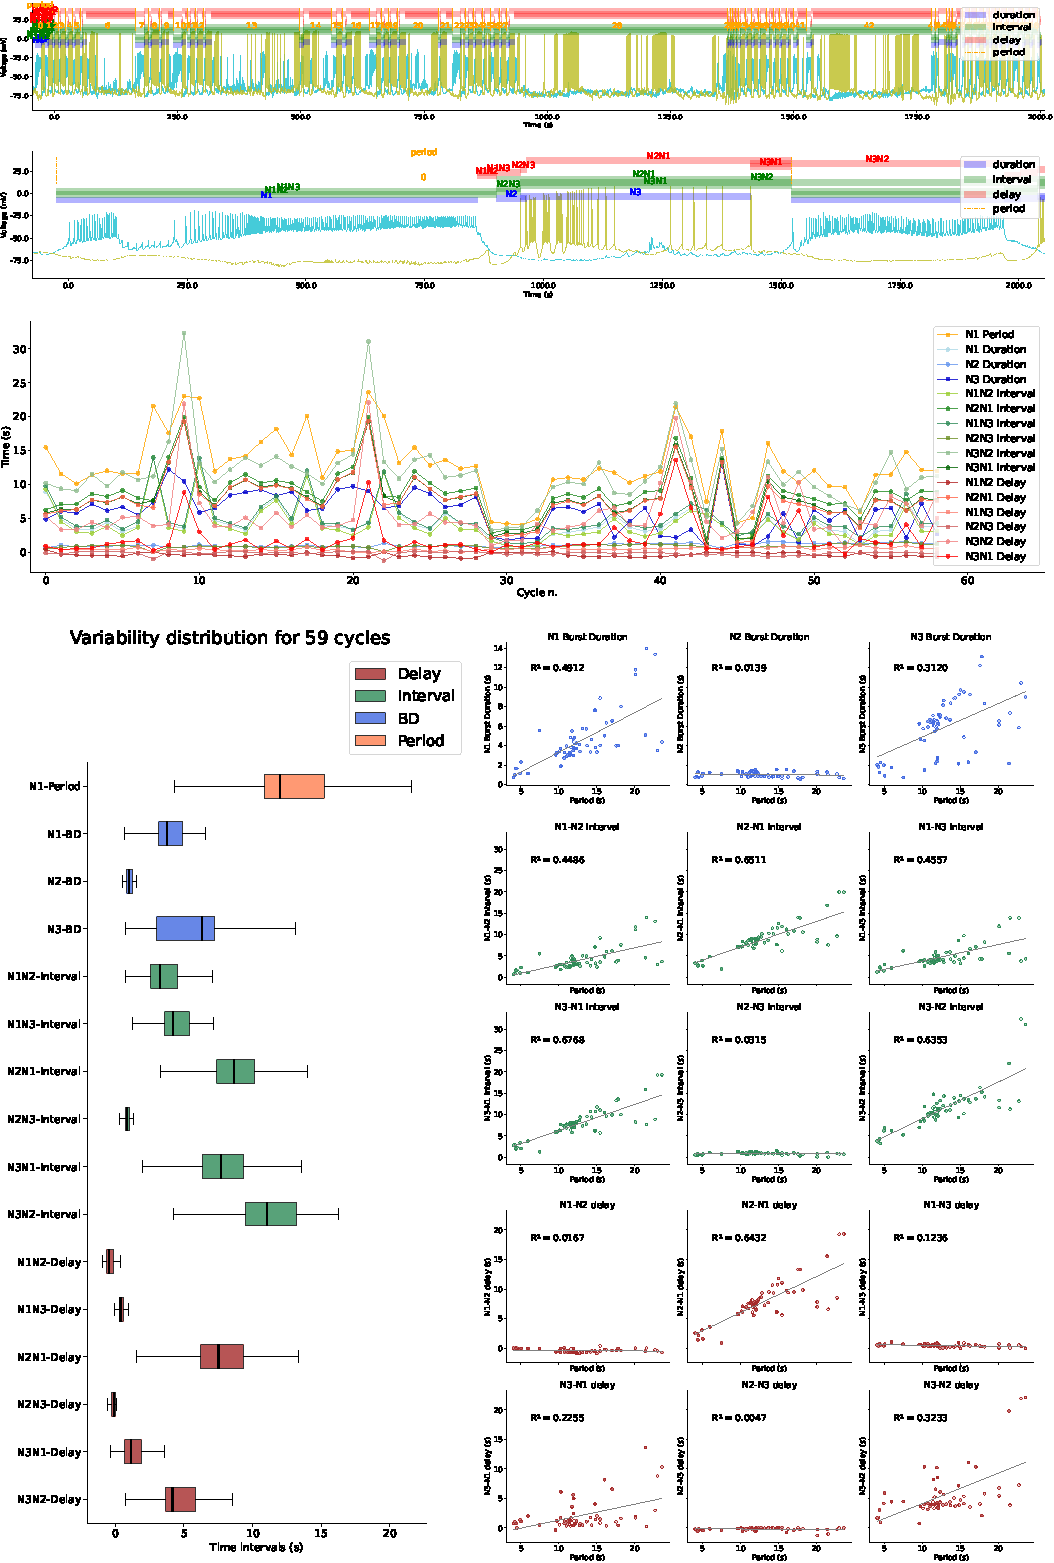
\includegraphics[width=\textwidth]{invariants/data/SUSSEX/prep3/images/3phases/panel_with_intervals.pdf}
		\end{column}
	\end{columns}
\end{frame}


\begin{frame}{SO driven activity}
	\begin{columns}
		\begin{column}{0.5\textwidth}
			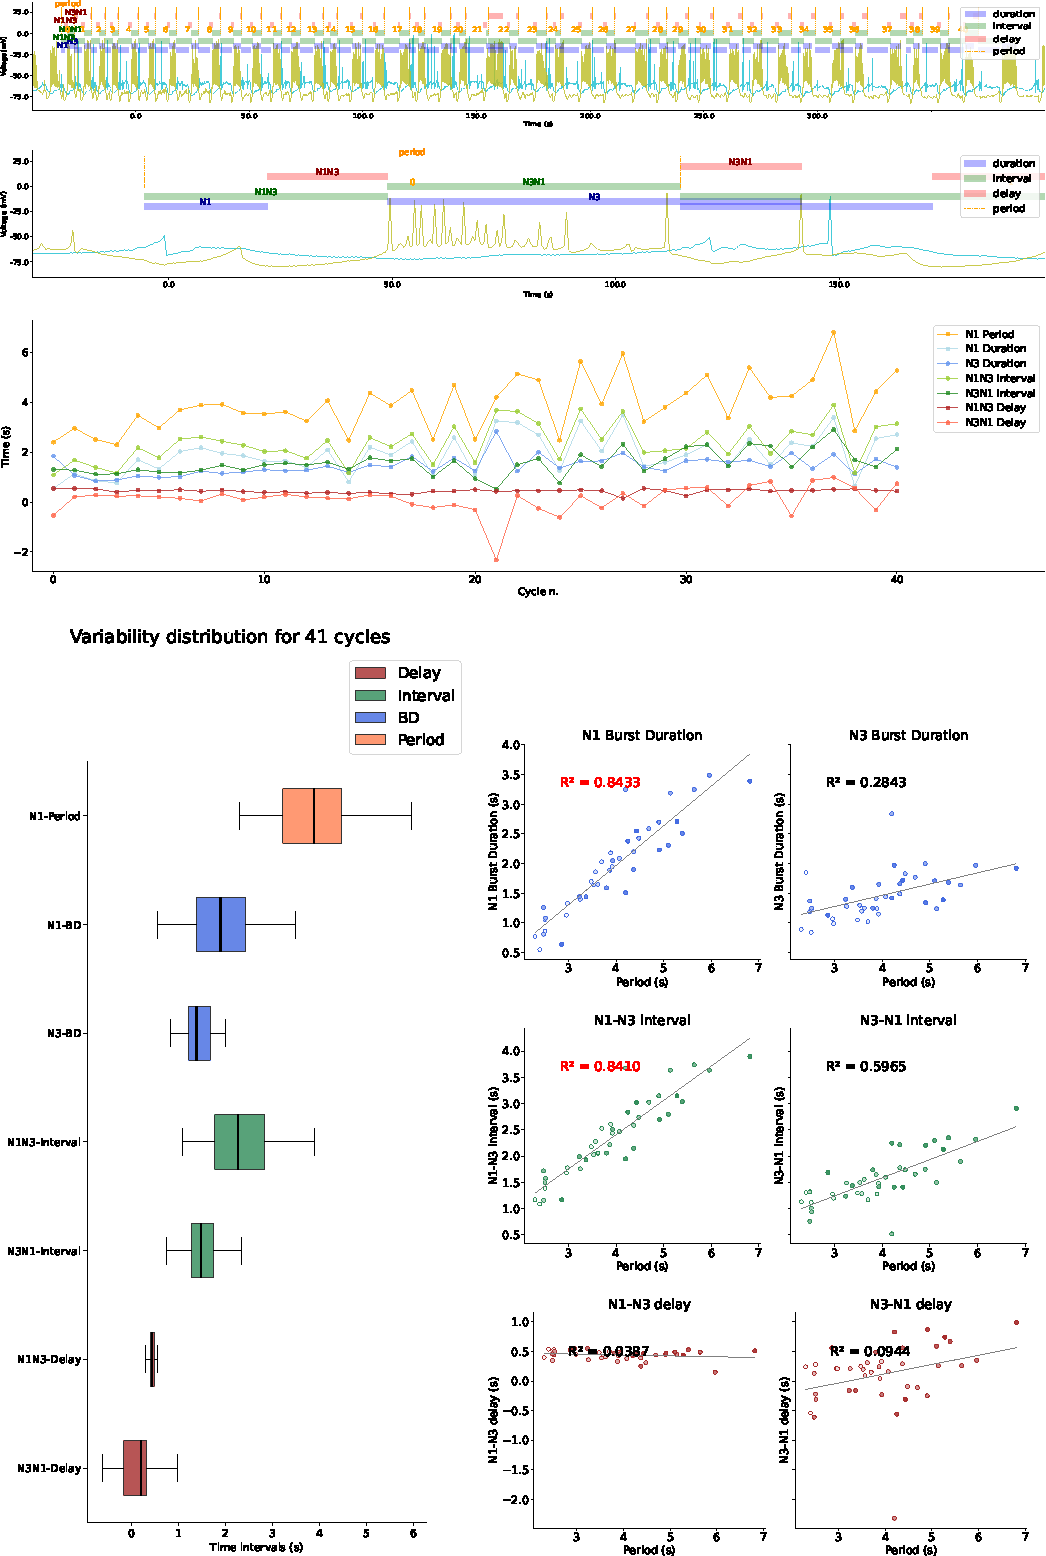
\includegraphics[width=\textwidth]{invariants/data/SUSSEX/SO_driven/images/panel_with_intervals.pdf}
		\end{column}
		\begin{column}{0.5\textwidth}
			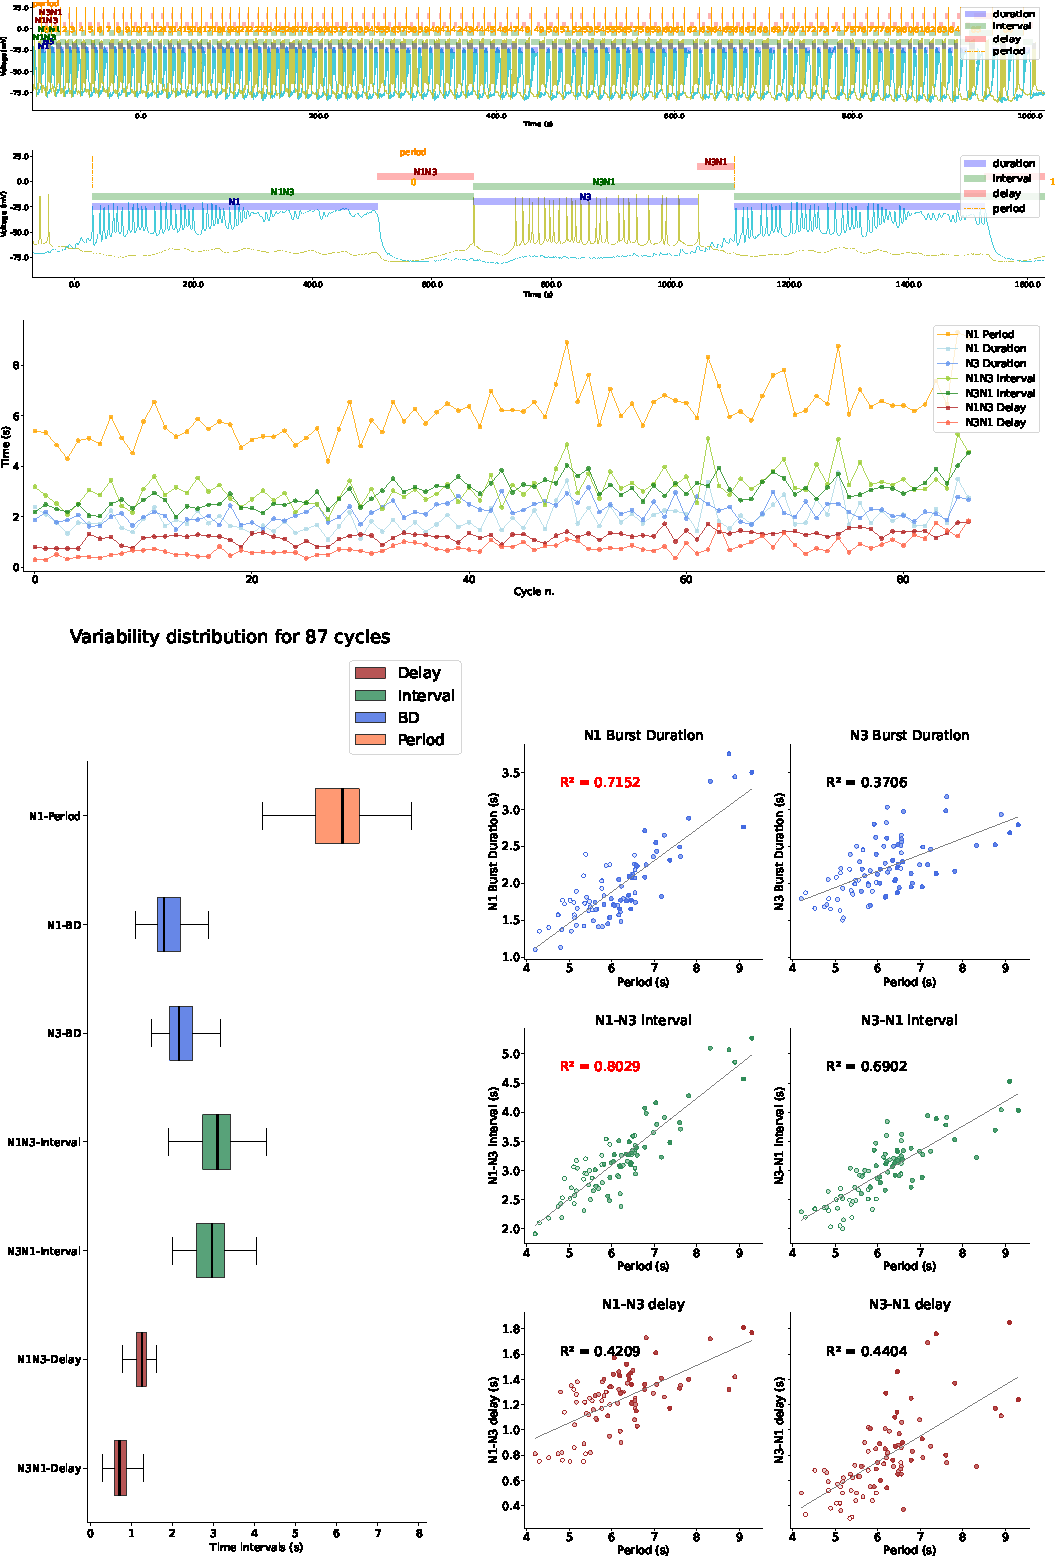
\includegraphics[width=\textwidth]{invariants/data/SUSSEX/prep4_so_driven_2/images/panel_with_intervals.pdf}
		\end{column}
	\end{columns}
\end{frame}



\begin{frame}{MLN driven activity}
	\begin{columns}
		\begin{column}{0.5\textwidth}
			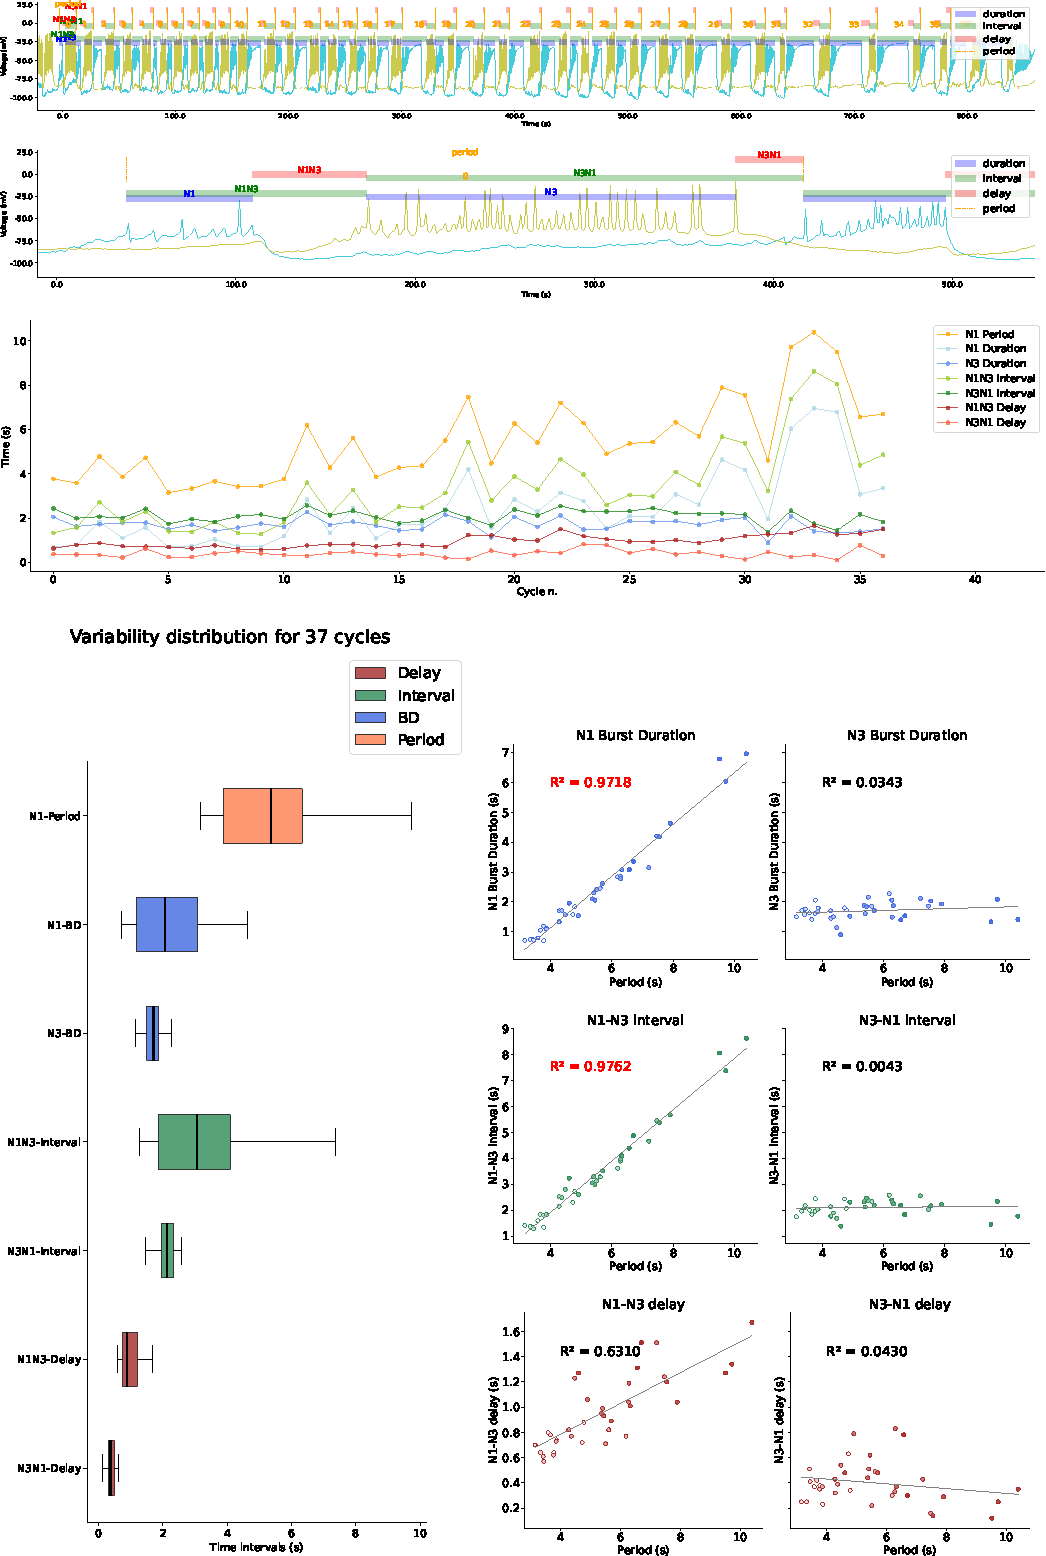
\includegraphics[width=\textwidth]{invariants/data/SUSSEX/MLN_driven/images/panel_with_intervals.pdf}
		\end{column}
	\end{columns}
\end{frame}

\begin{frame}{CV1 driven activity}
	\begin{columns}
		\begin{column}{0.5\textwidth}
			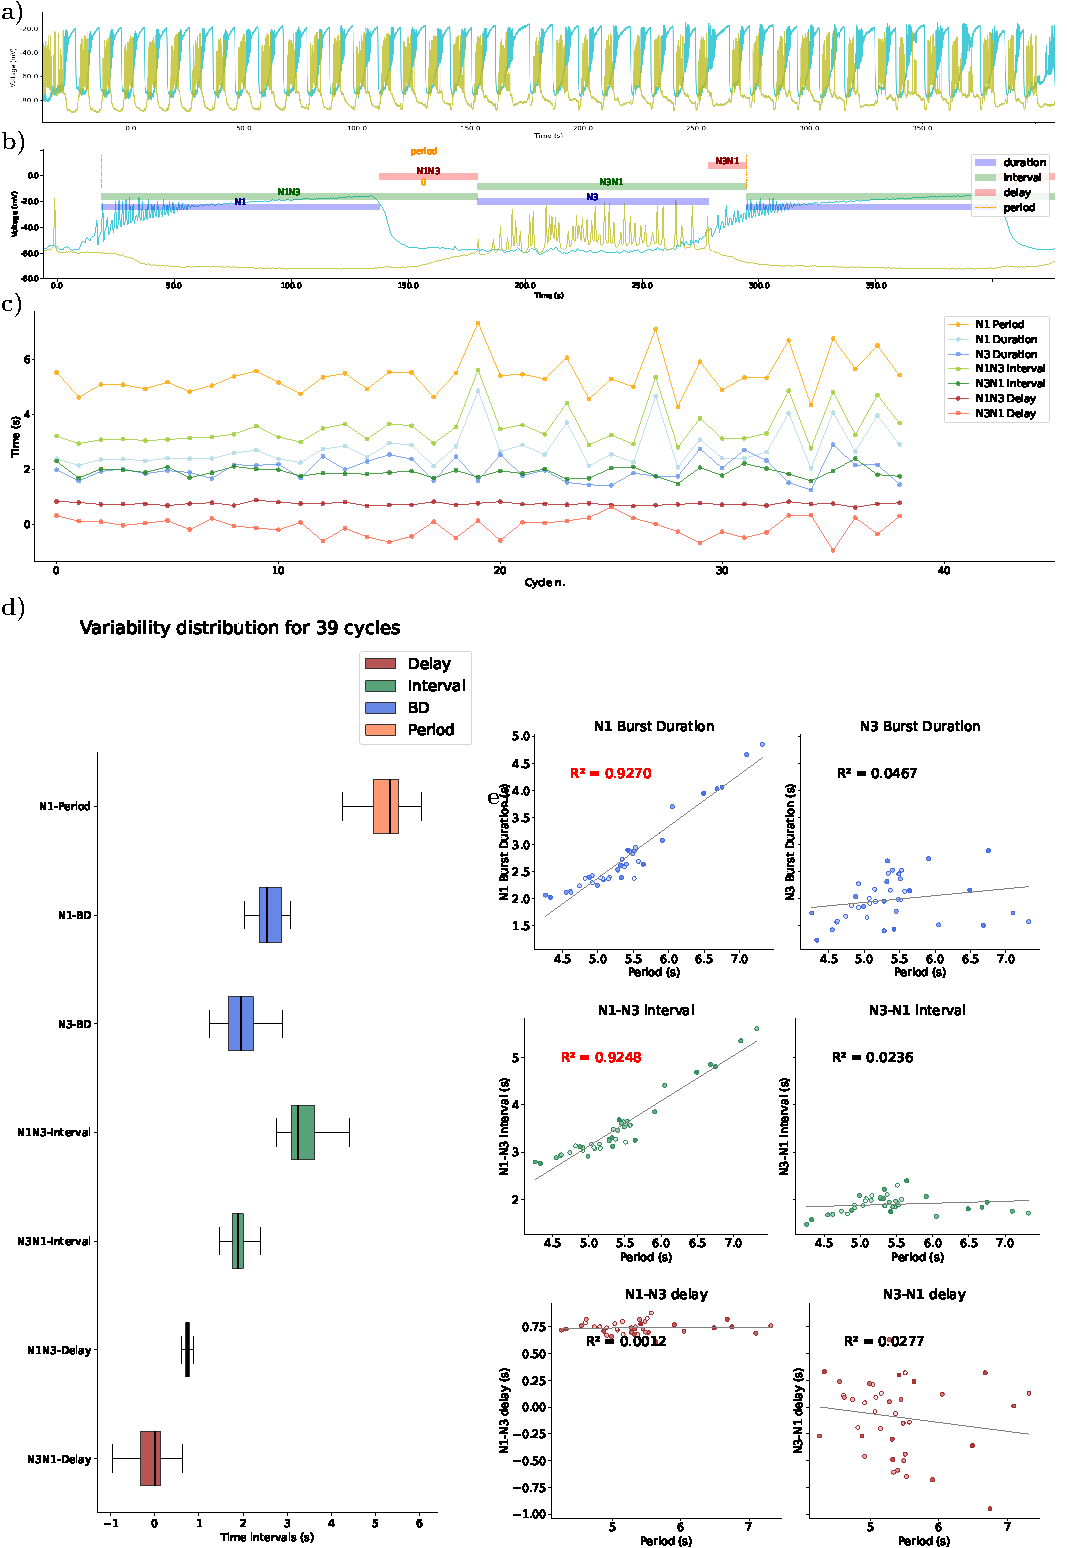
\includegraphics[width=\textwidth]{invariants/data/SUSSEX/CV1a_driven1/images/2phases/panel_with_intervals.pdf}
		\end{column}
		\begin{column}{0.5\textwidth}
		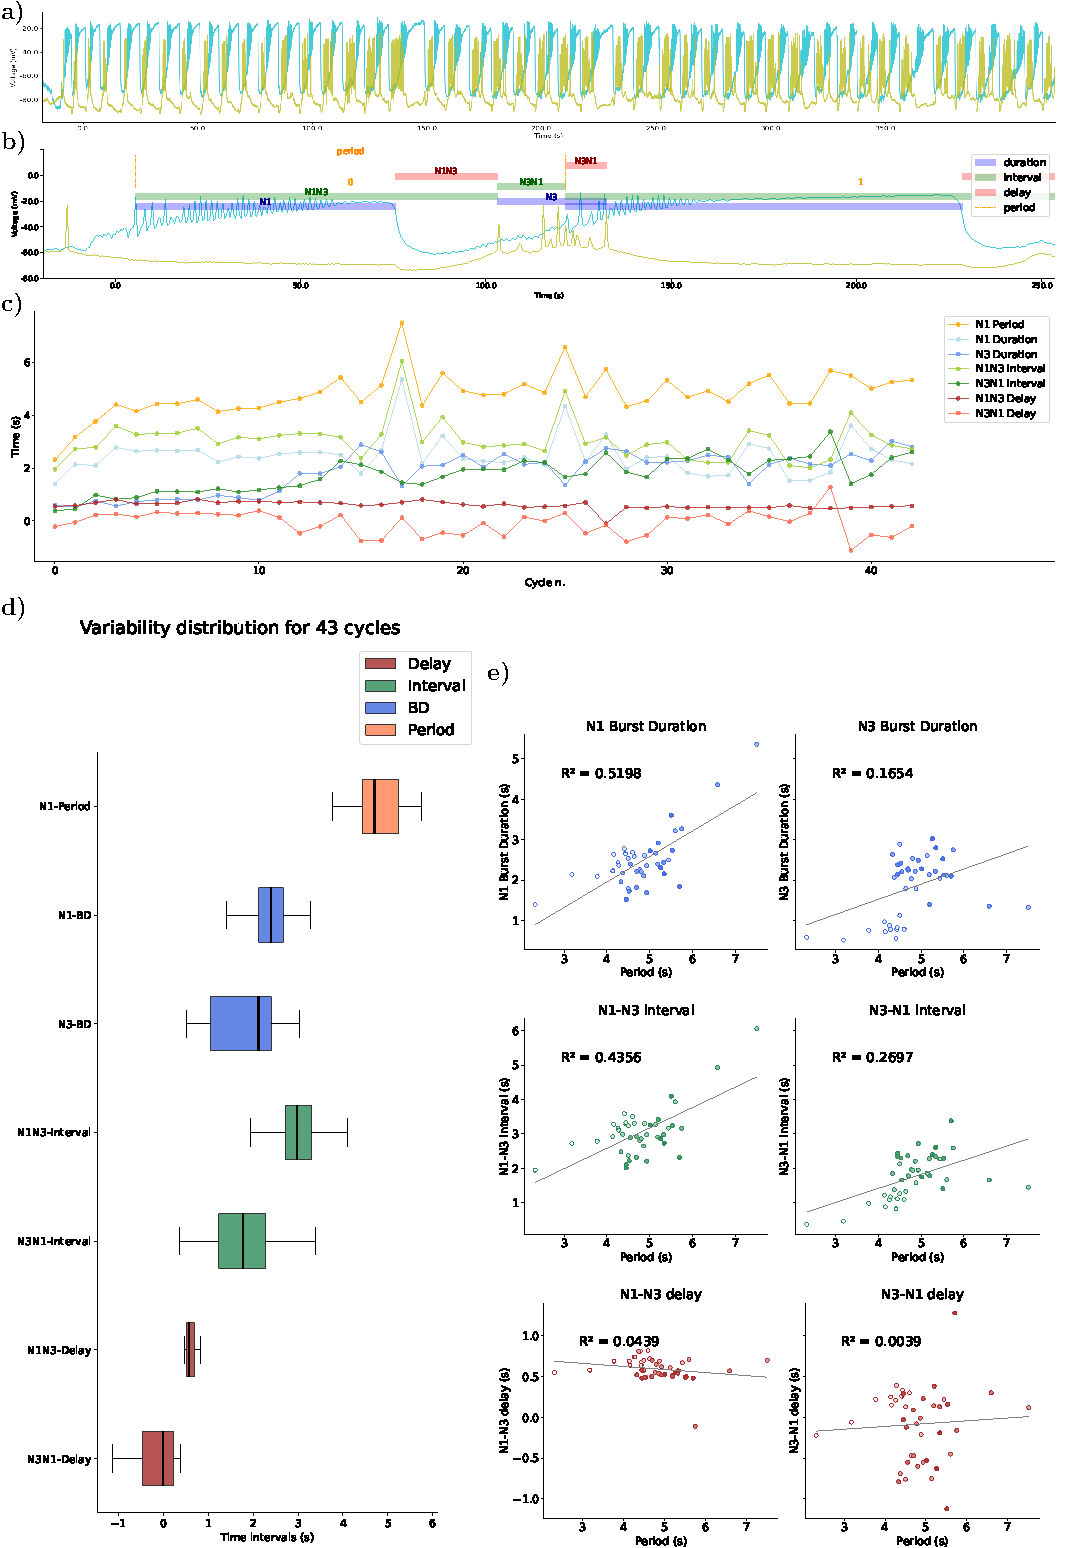
\includegraphics[width=\textwidth]{invariants/data/SUSSEX/CV1a_driven2/images/panel_with_intervals.pdf}
		\end{column}
	\end{columns}
\end{frame}

\begin{frame}{Robot}
%	\begin{figure}[h!]
%		\centering
%		\href{https://youtu.be/ny2dJGbG8lo&t=120s}{
%			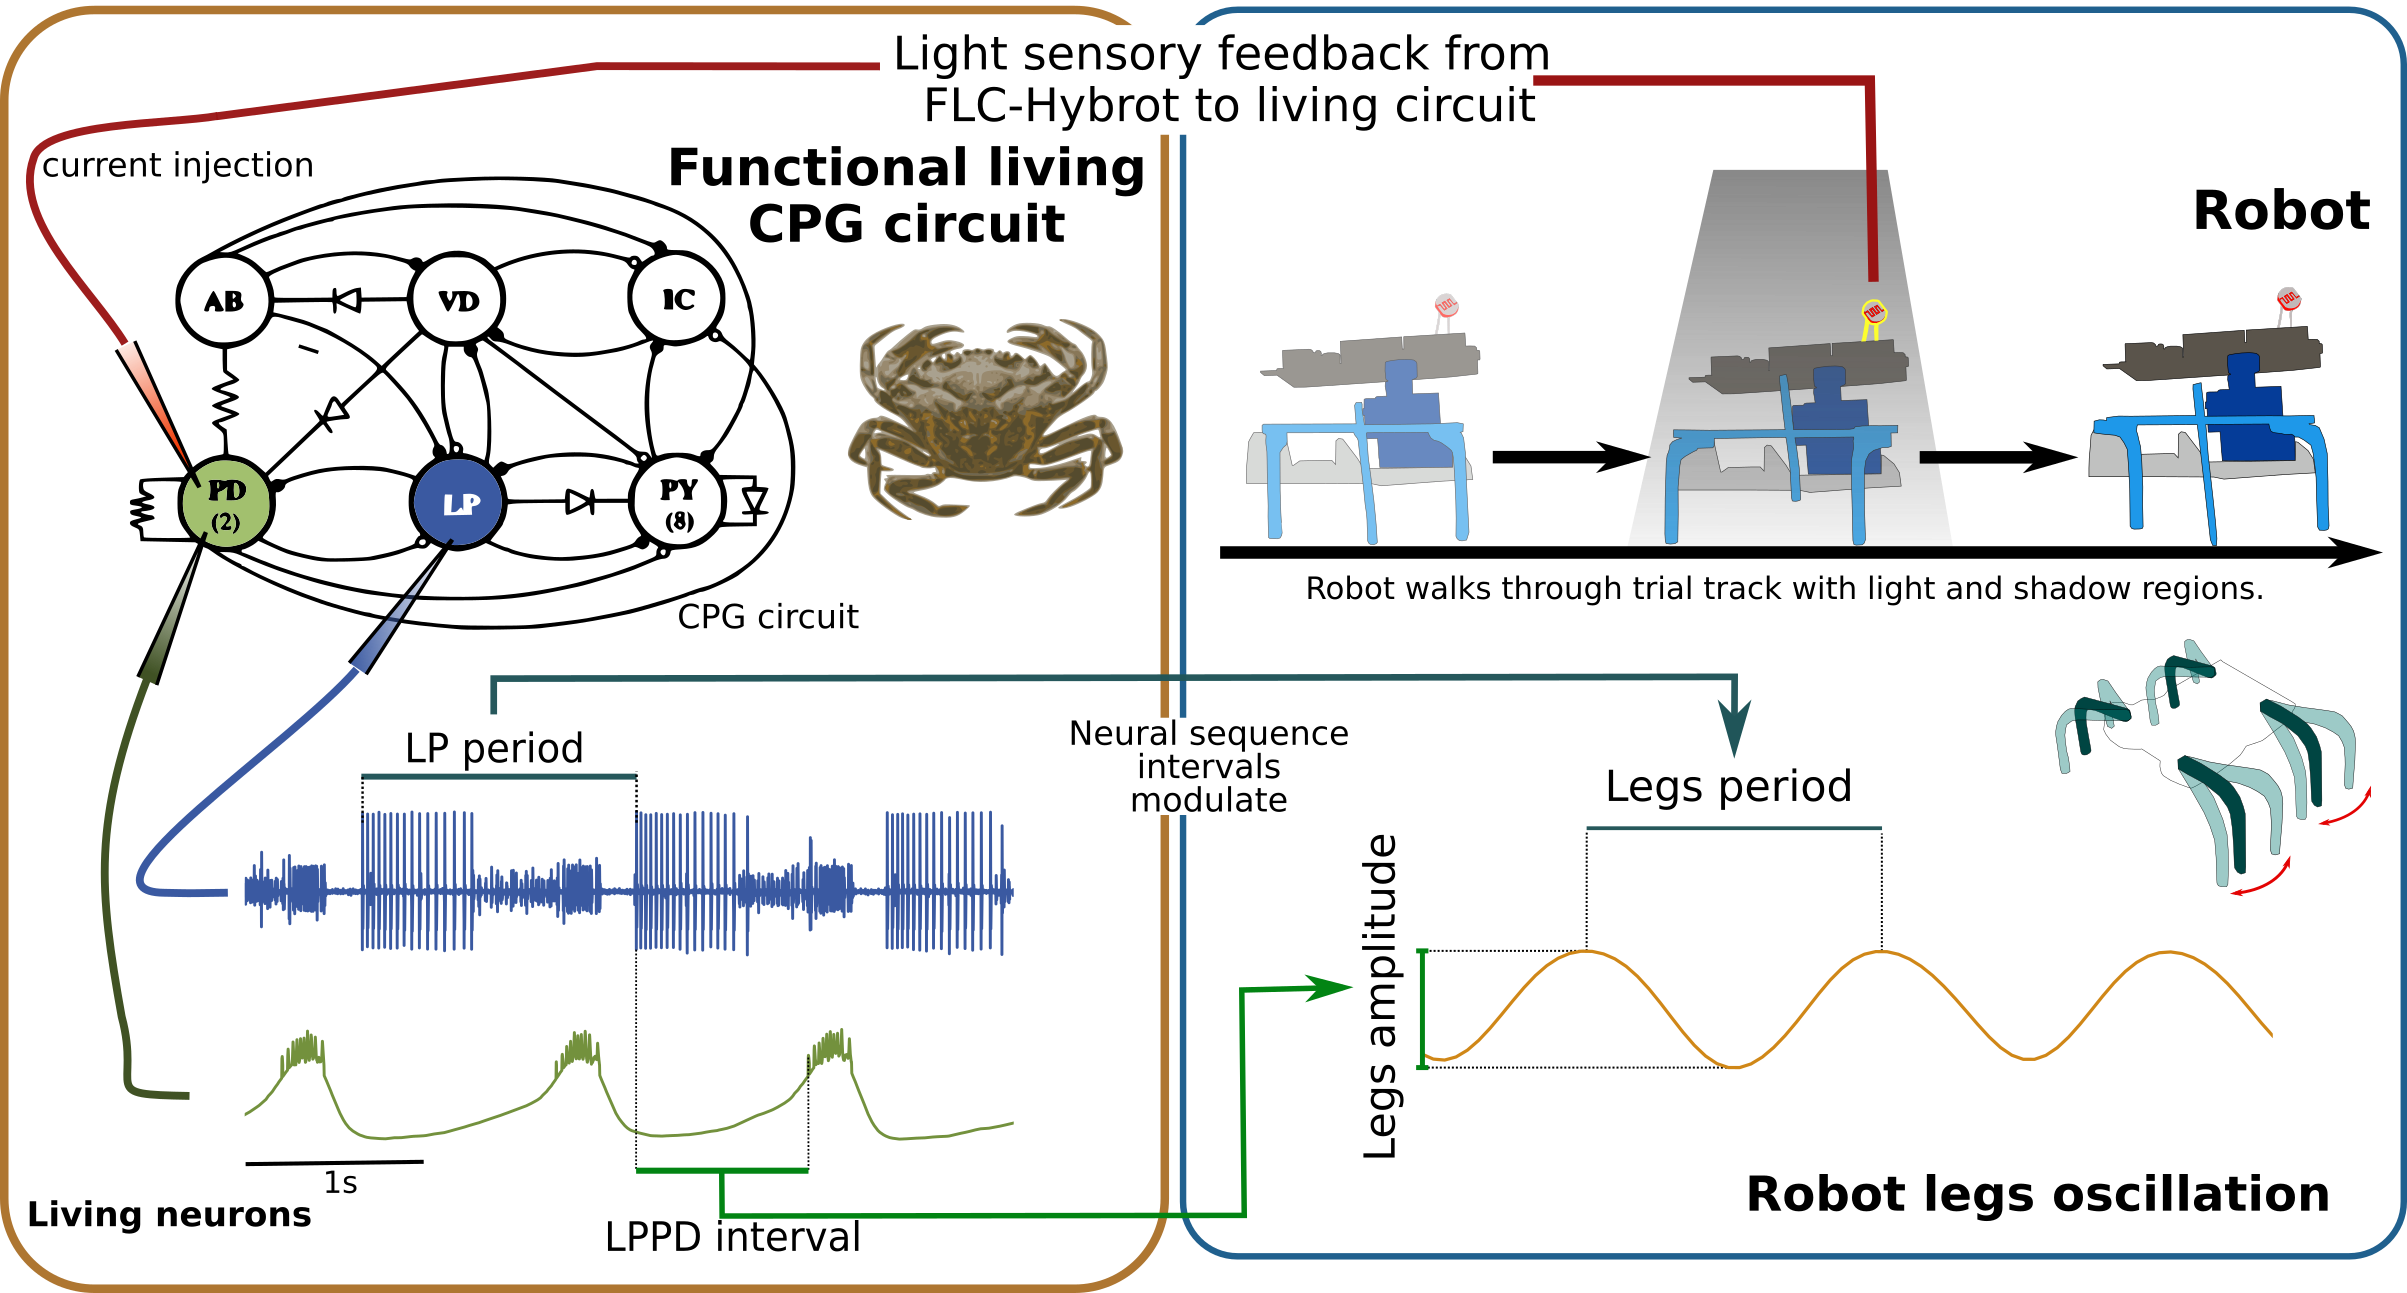
\includegraphics[width=\textwidth]{invariants/robot/Figure1_experiment_design_v1.png}
%		}
%		\caption{Pyloric video starting at 2 minutes}
%	\end{figure}

	\includemedia[
	width=\textwidth,
	height=0.5625\textwidth,  % 16:9 aspect ratio
	activate=pageopen,
	flashvars={
		modestbranding=1 % no YouTube logo in control bar
		autoplay=1
		&rel=0 % don't show related videos
	}
]{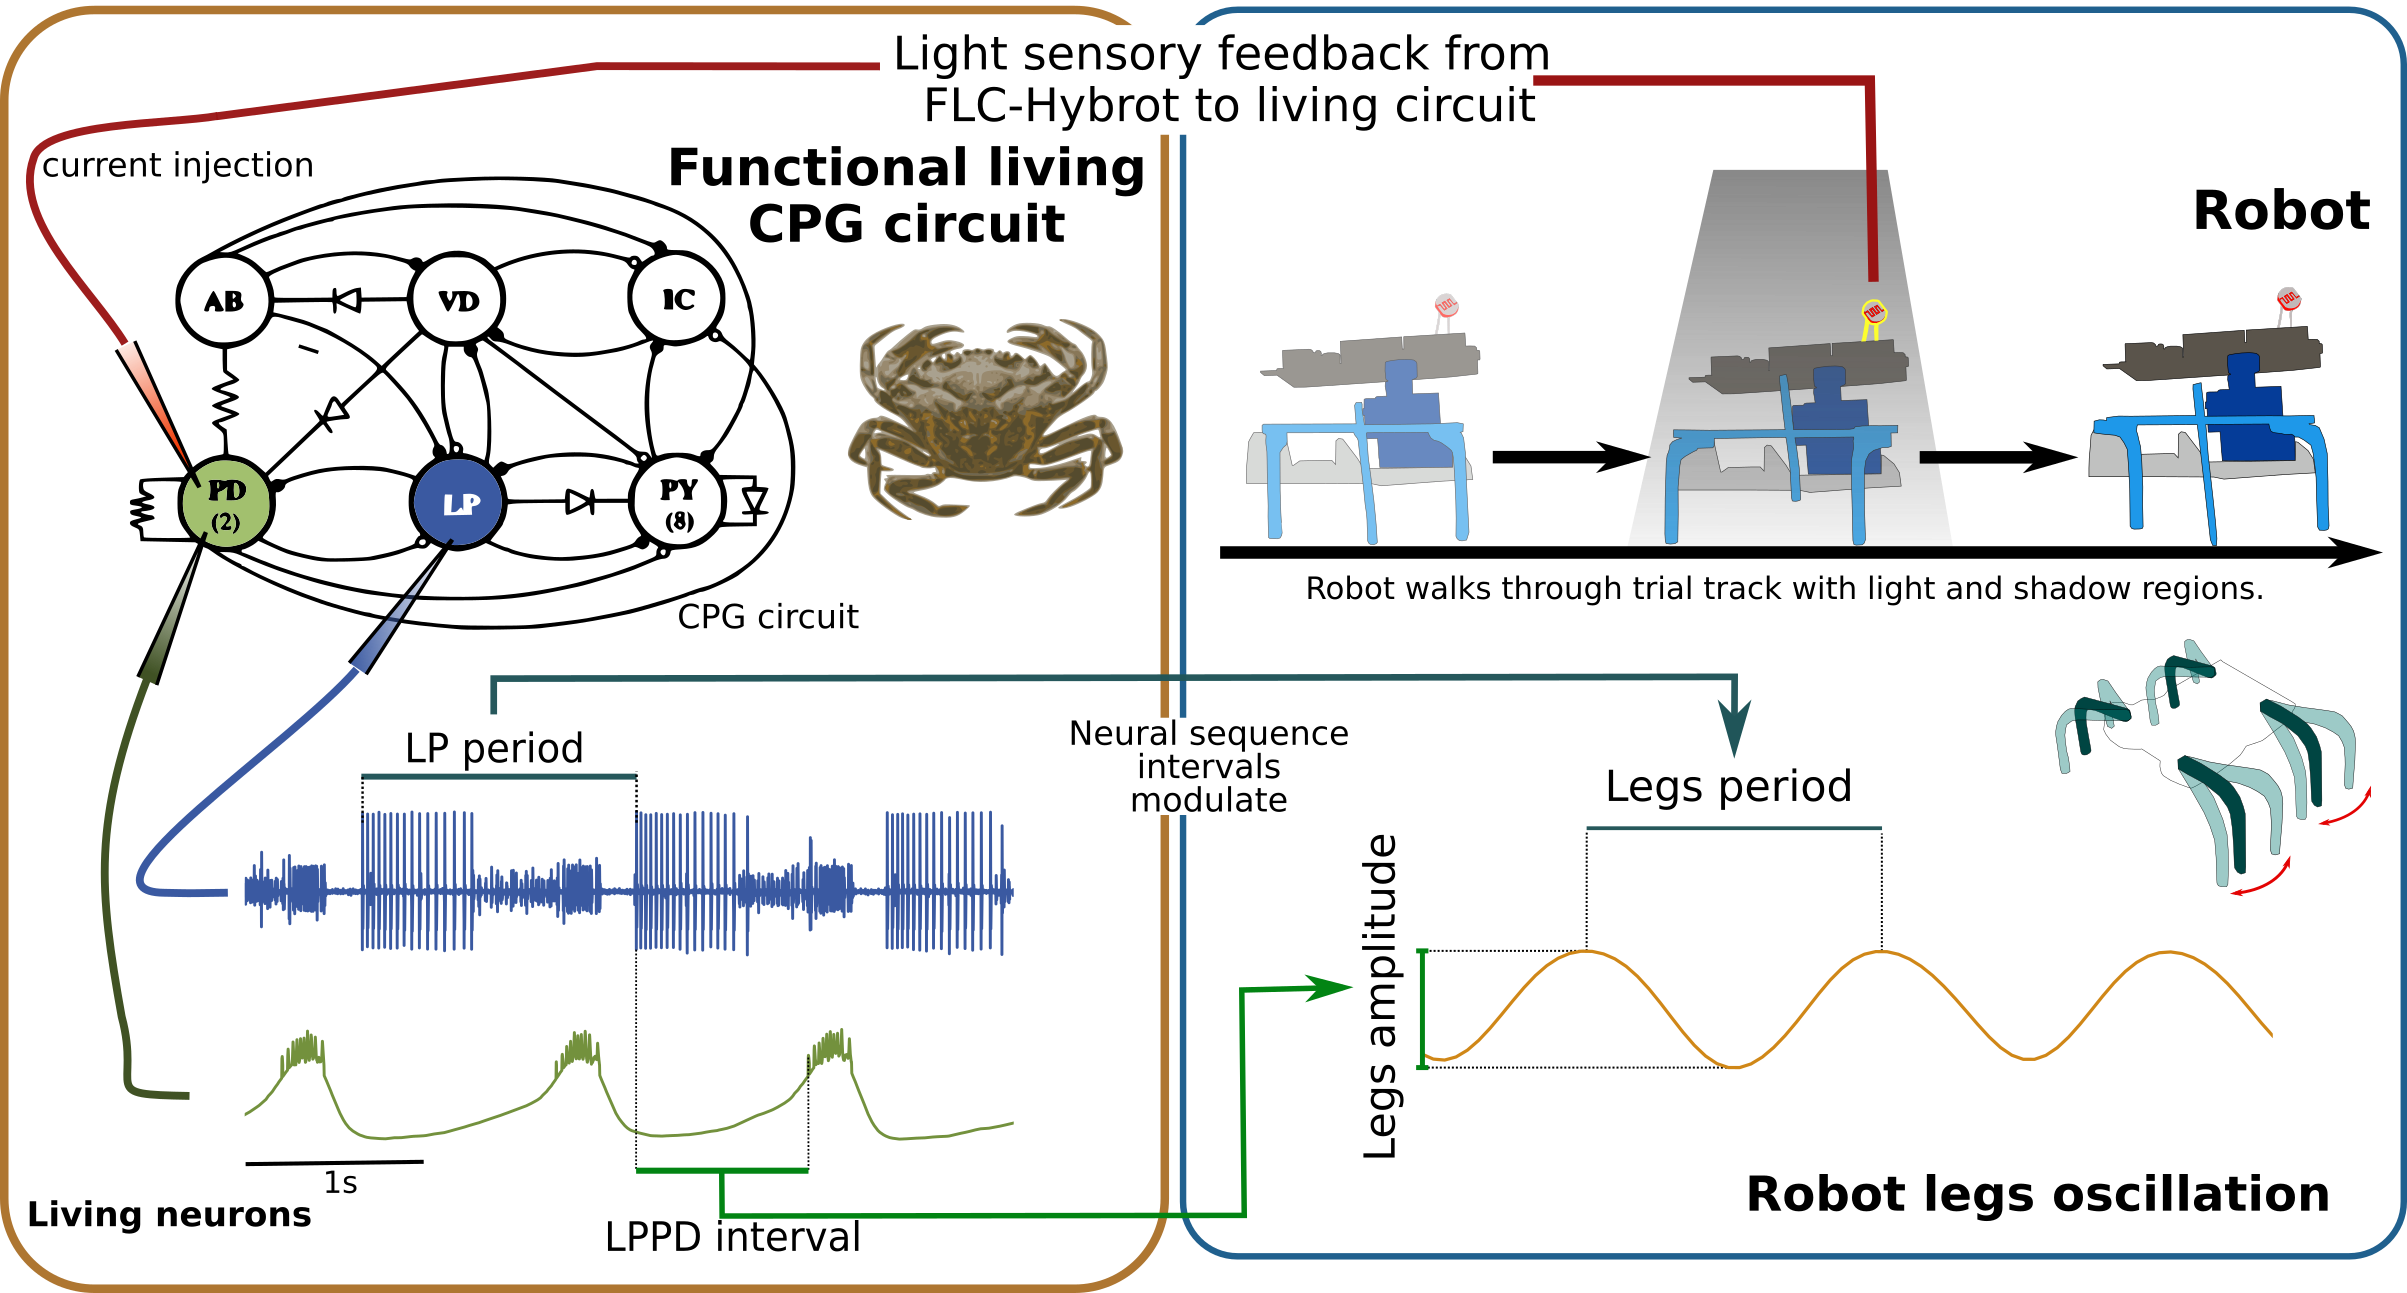
\includegraphics{invariants/robot/Figure1_experiment_design_v1.png}}{https://youtu.be/ny2dJGbG8lo}
%	]{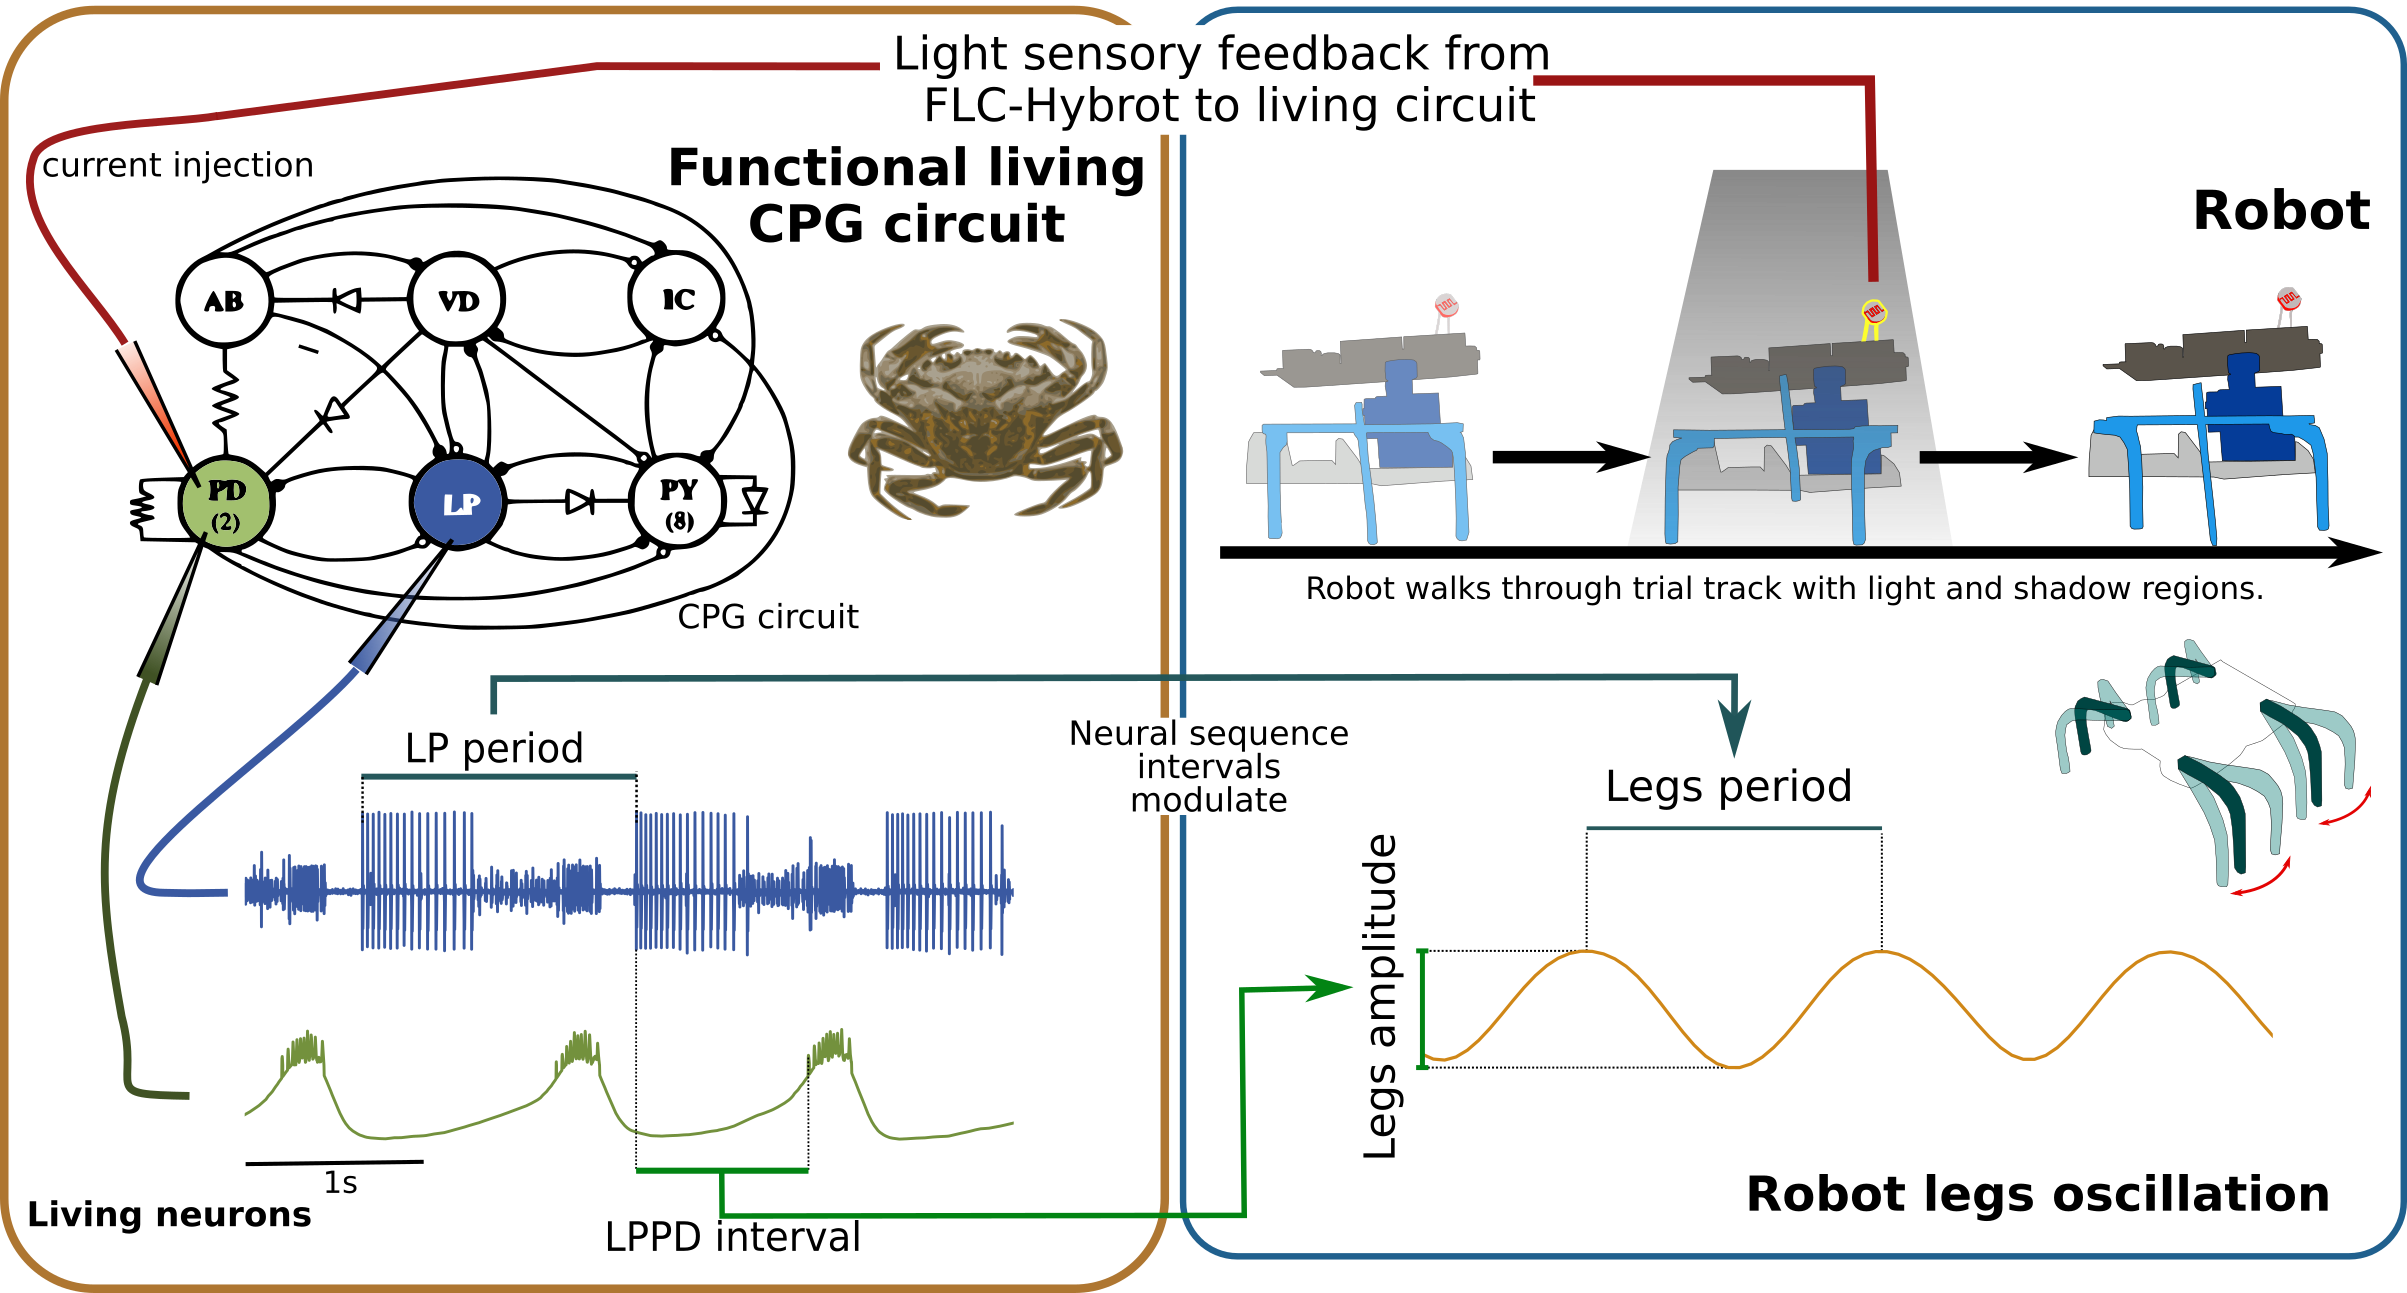
\includegraphics{invariants/robot/Figure1_experiment_design_v1.png}}{https://youtu.be/ny2dJGbG8lo&t=120s}
%\caption{Robot demo}
\end{frame}


\section[CW-NIR Neuromodulation]{CW-NIR laser as an effective neuromodulation technique}
\begin{frame}{Current findings}
\end{frame}
\begin{frame}{Experimental setup}
	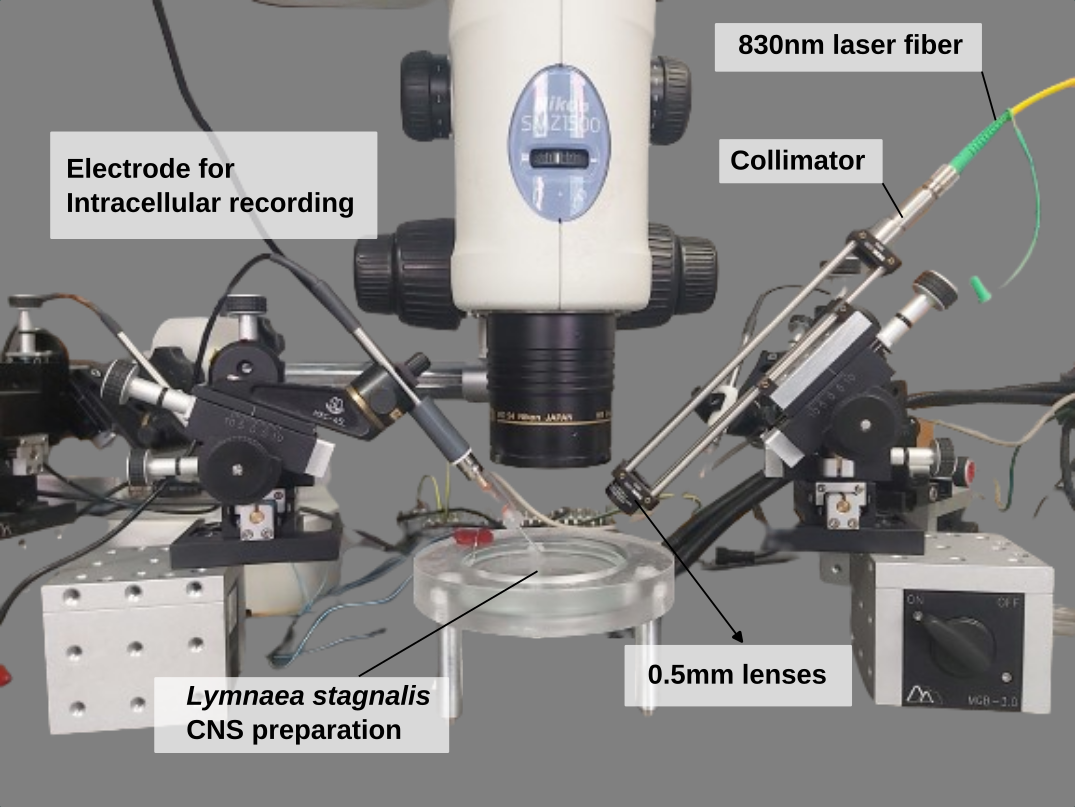
\includegraphics[width=\textwidth]{methods/laser-setup_labels.png}
\end{frame}


\begin{frame}{Effect on single neurons dynamics}
\end{frame}


\begin{frame}{Modulation of the spike waveform}
	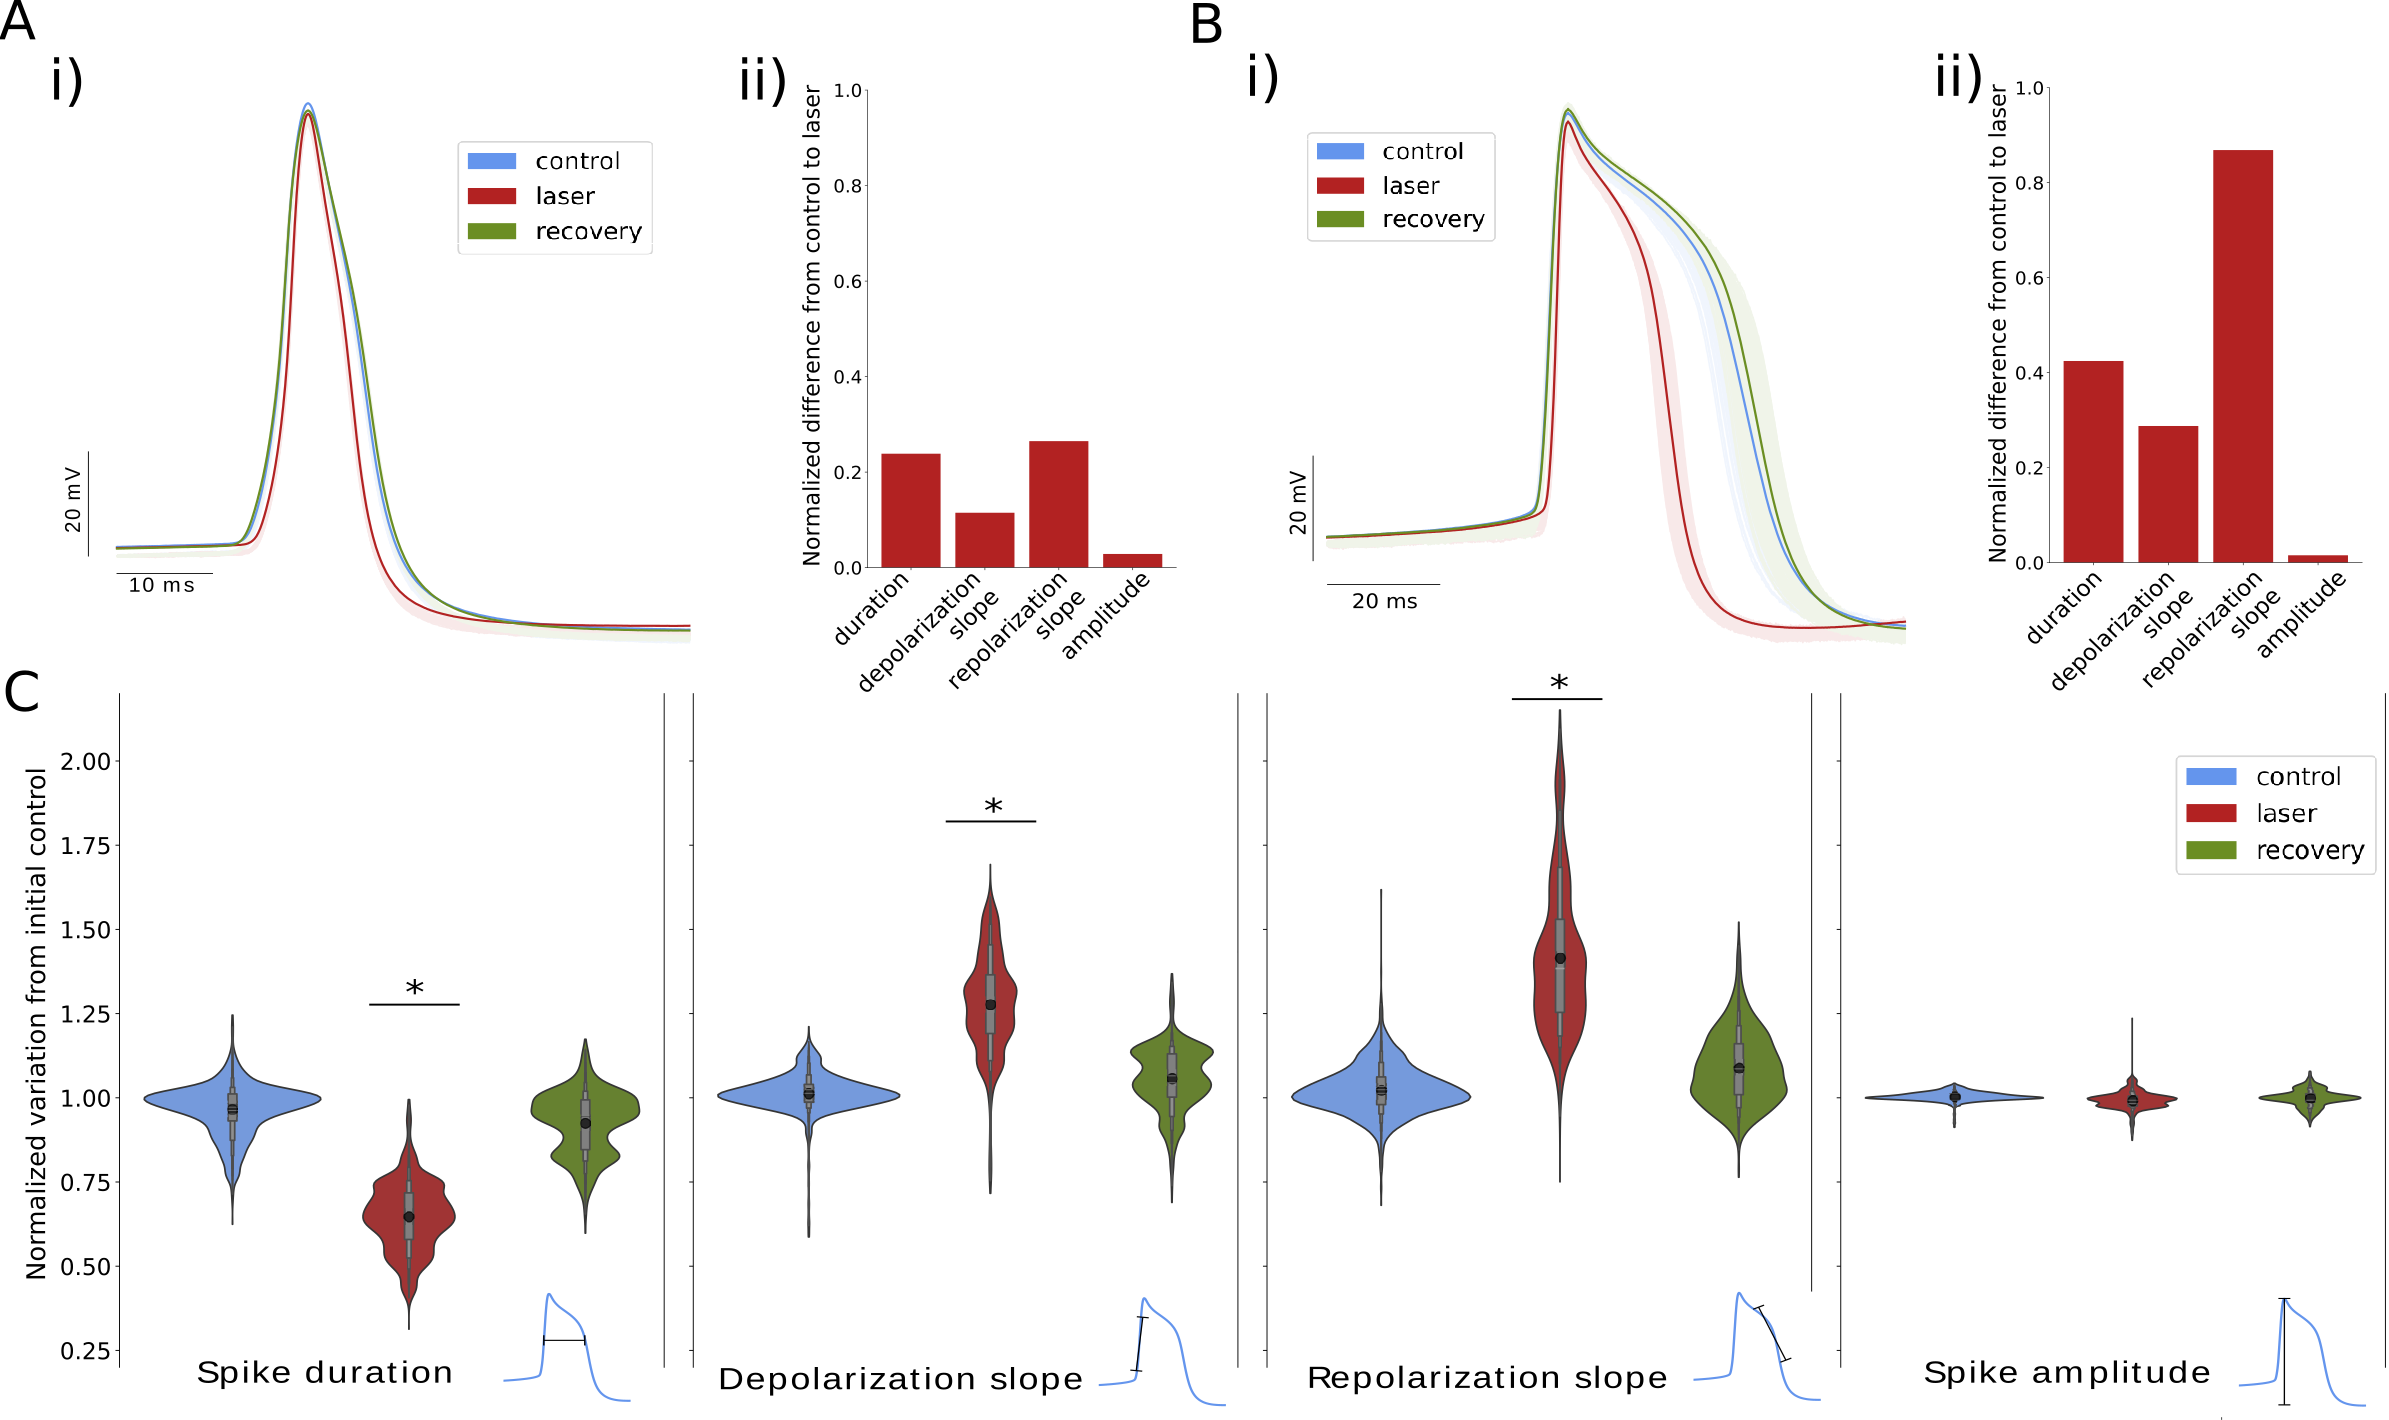
\includegraphics[width=\textwidth]{laser/Figure2.png}
\end{frame}

\begin{frame}{Effect on the firing rate}
	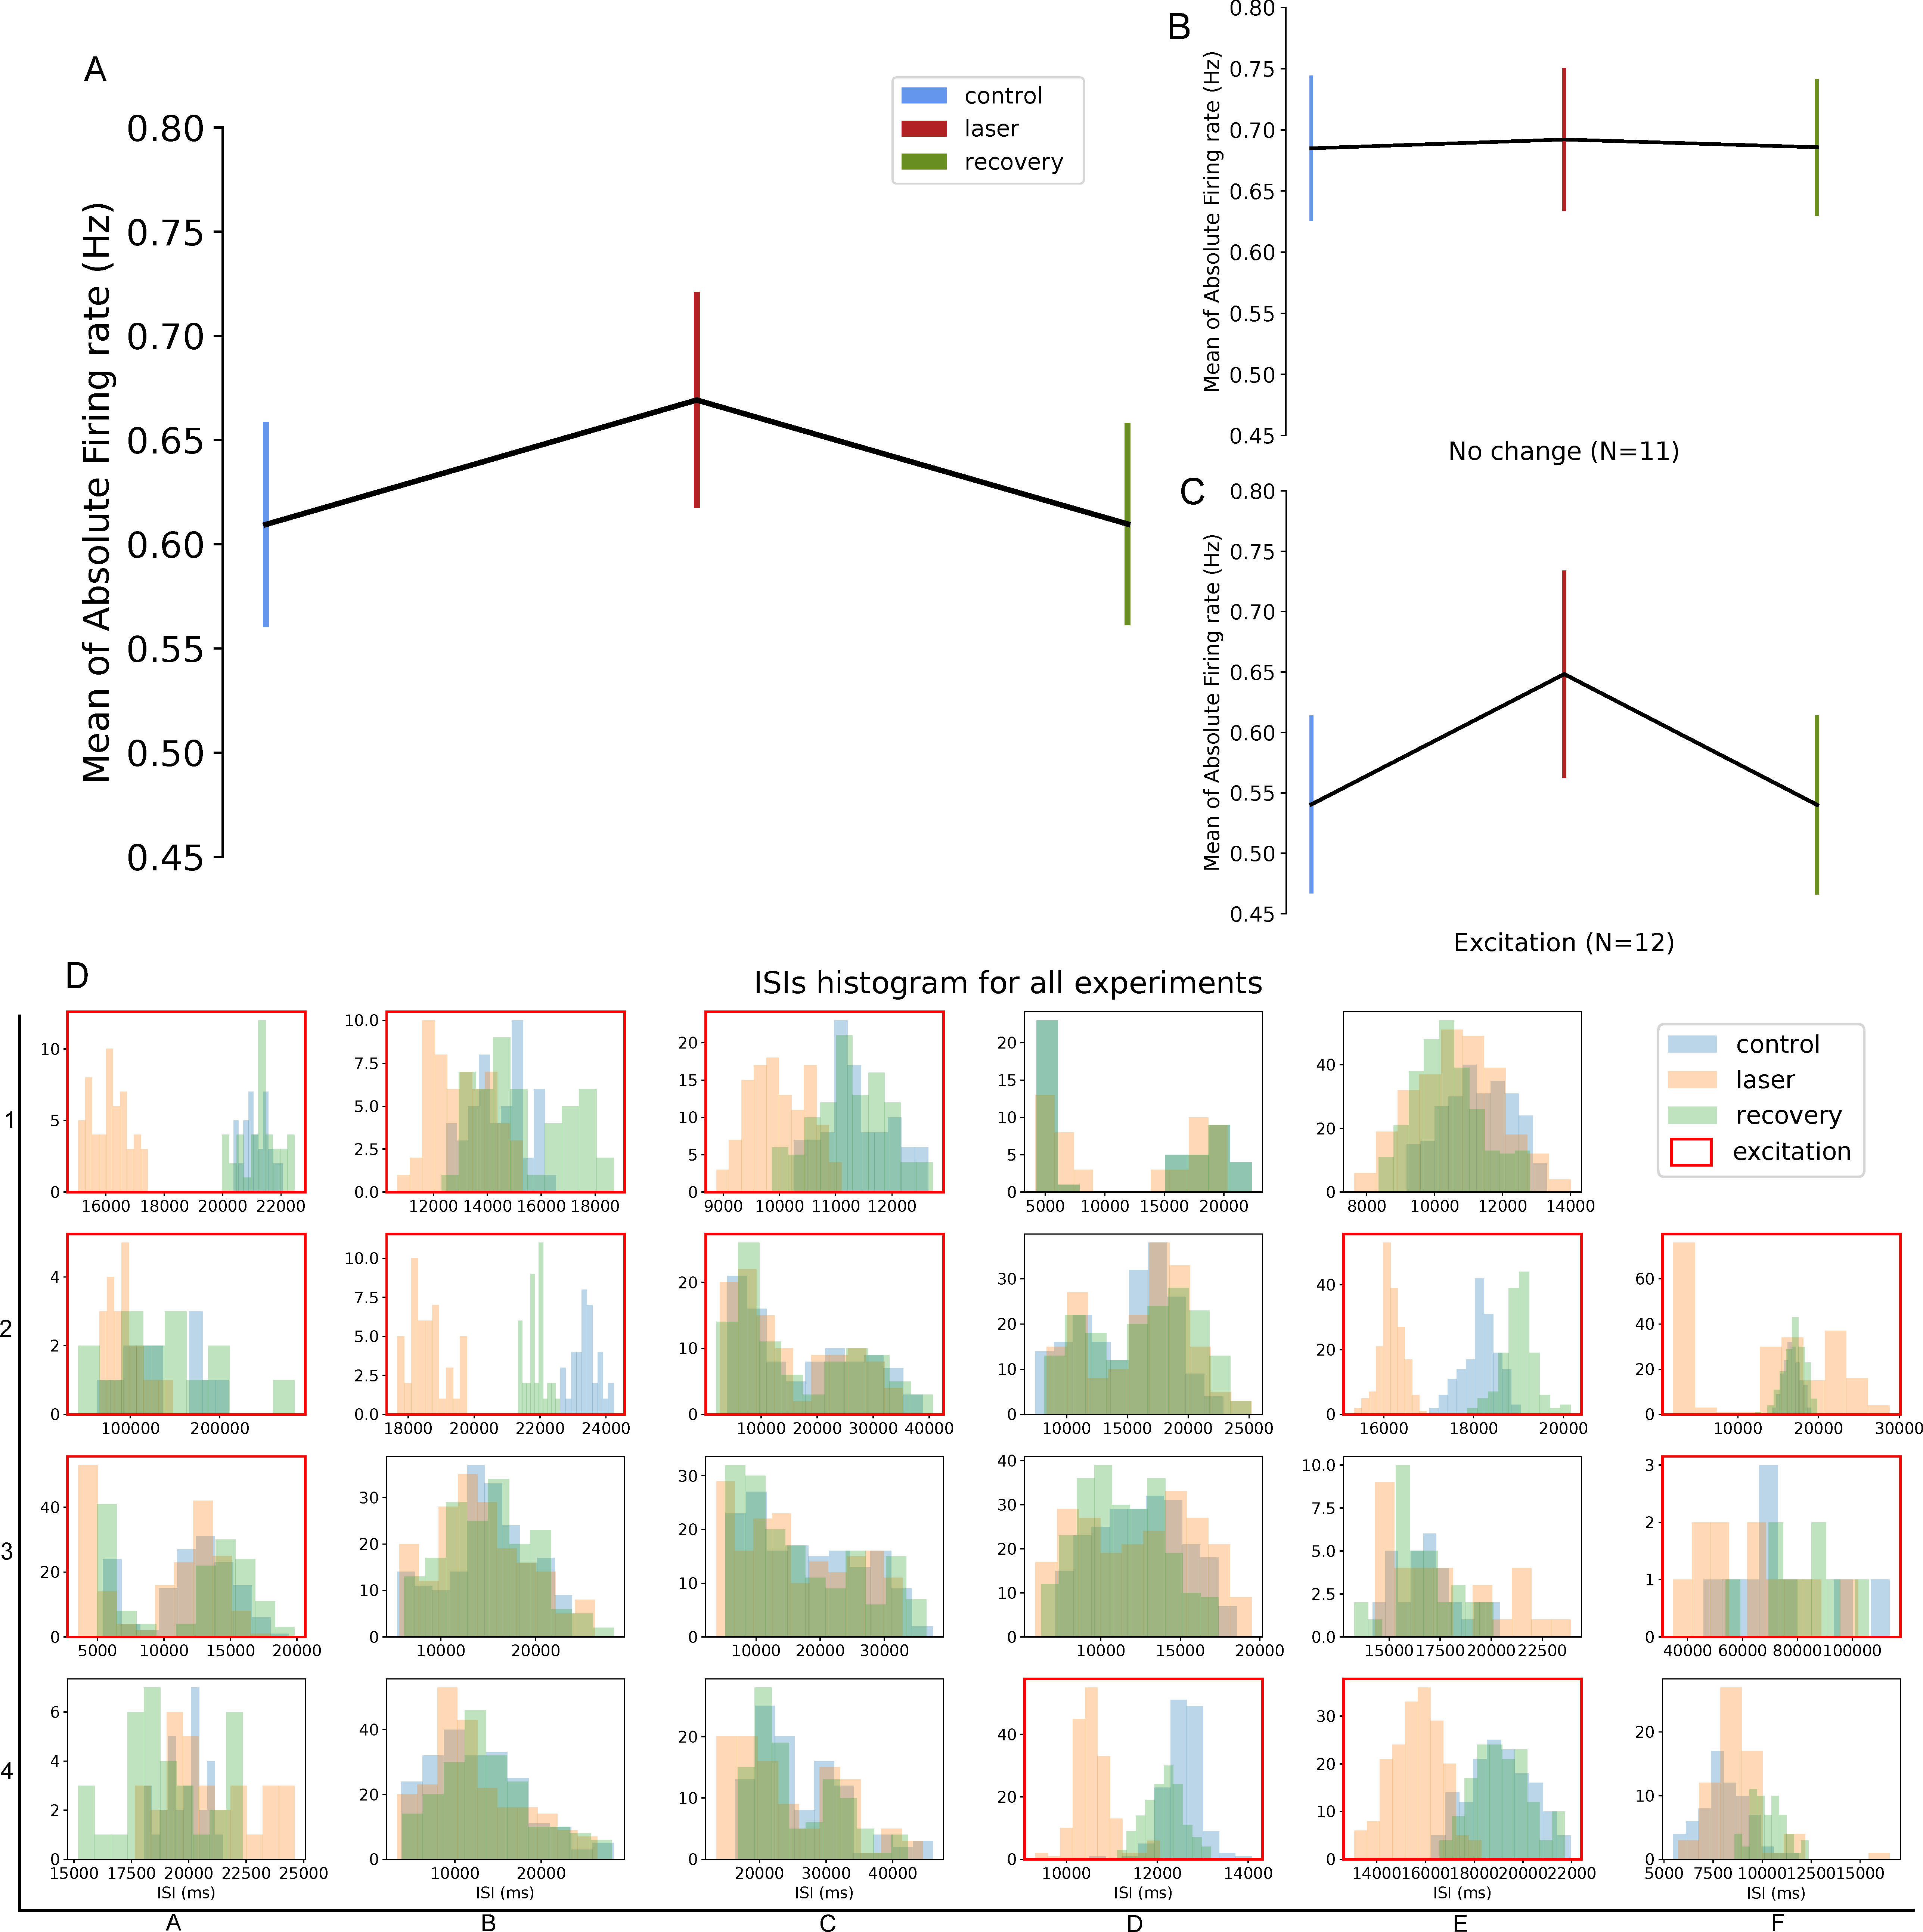
\includegraphics[width=\textwidth]{laser/frequency.pdf}
\end{frame}


\begin{frame}{Effect on a minimal circuit}
	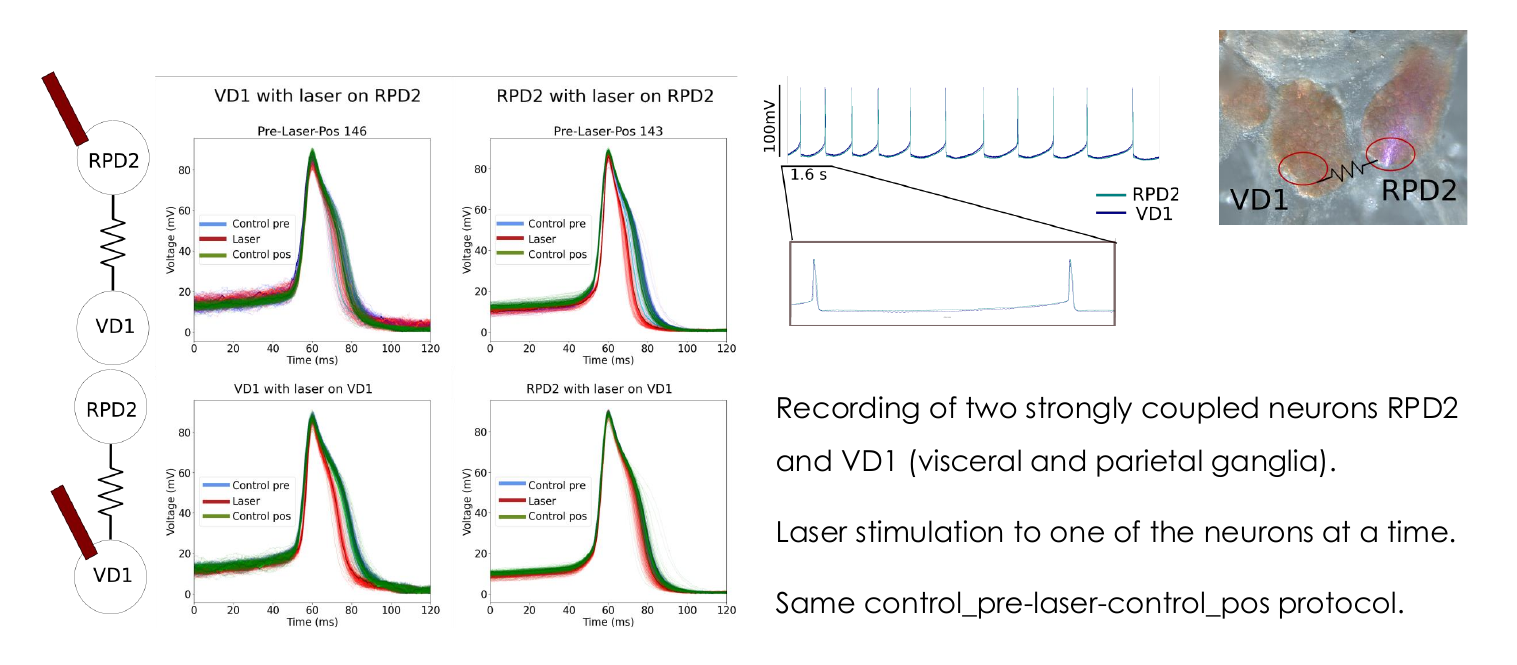
\includegraphics[width=\textwidth]{Images/electrical.png}
\end{frame}


\begin{frame}{Model analysis to explore candidates}
\end{frame}

\begin{frame}{Model with temperature description}
\end{frame}


\begin{frame}{Activity-dependent stimulation}
\end{frame}


\section{Conclusion}

    \begin{frame}{Conclusion}
    \end{frame}
%}
%\setbeamercolor{background canvas}{bg=violet}
\setbeamercolor{background canvas}{bg=CCNUMaize}
\begin{frame}[plain,t]
\vspace{100pt}
\centering

\includegraphics[width=0.6\textwidth]{logos/UAM+EPS_L-eps-converted-to.pdf}
\end{frame}
\end{document}